\documentclass[b5paper]{report}

% \usepackage{titlesec}
% \titleformat{\chapter}[display]
%   {\Large\bfseries}
%   {\chaptertitlename\ \thechapter}{0pt}{\Huge}

\usepackage[Lenny]{fncychap}
\usepackage[style=ieee, citestyle=numeric-comp, backend=biber]{biblatex}
\addbibresource{refs.bib}

% \usepackage[T1]{fontenc}
% \usepackage{titlesec, blindtext, color}
% \definecolor{gray75}{gray}{0.75}
% \newcommand{\hsp}{\hspace{20pt}}
% \titleformat{\chapter}[hang]{\Huge\bfseries}{\thechapter\hsp\textcolor{gray75}{|}\hsp}{0pt}{\Huge\bfseries}


\usepackage{graphicx}
\usepackage{mwe}

\usepackage{skeldoc}
\usepackage{pseudo}
\usepackage{tcolorbox}
\usepackage{tabto}


\usepackage{jlcode}

\usepackage{caption}
\usepackage{threeparttable}

\usepackage{amsmath}
\usepackage{amssymb}

\usepackage[page,toc,titletoc,title]{appendix}
\usepackage{hyperref}

\usepackage{epigraph}

\usepackage{tikz}
\usetikzlibrary{backgrounds}
\usetikzlibrary{positioning}

\definecolor{lighttan}{cmyk}{0,0.05,0.17,0}
\definecolor{darktan}{cmyk}{0,0.07,0.26,0.06}
% \definecolor{complementaryblue}{RGB}{177,194,240}
\definecolor{complementaryblue}{RGB}{202,226,248}
\definecolor{averagegreen}{RGB}{214,232,205}

\pseudoset{label=\small\arabic*, hd-space}

\tcbuselibrary{skins,theorems}
\newtcbtheorem{algorithm}{Algorithm}{pseudo/ruled}{alg}
\TabPositions{2cm}

\setlength\epigraphwidth{.5\textwidth}

\begin{document}

\newcommand{\mono}[1]{$\texttt{#1}$}

\begin{titlepage}
  \newcommand{\HRule}{\rule{\linewidth}{0.5mm}}

  \vbox{ }
  \vbox{ }
  \begin{center}
    % Upper part of the page
    
\includegraphics[width=0.15\textwidth]{ntnu.png}\\[1cm]
    \textsc{\Large Department of Computer Science}\\[1.5cm]
    \textsc{\large TDT4900 --- Master's thesis}\\[0.5cm]
    \vbox{ }

    % Title
    \HRule \\[0.4cm]
    { \huge Exploring Matroids in Fair Allocation:}\\[0.1cm]
    { \huge Building the Matroids.jl Library}\\[0.1cm]
    \HRule \\[1.5cm]

    % Author
    \large
    \emph{Author:}\\
    Andreas Aaberge Eide\\[0.5cm]
    \emph{Supervisor:}\\
    Magnus Lie Hetland
    \vfill

    % Bottom of the page
    {\large \today\par}
  \end{center}
\end{titlepage}


\epigraph{In matroid theory, we explore

A structure with properties galore

From bases to circuits

It never discourages

Mathematicians always wanting more
\newline
\newline
The axioms it holds are so grand

And its applications vast and unplanned

From optimization to graphs

It can solve so many tasks

Matroid theory, truly a wonderland}{ChatGPT}
\thispagestyle{empty}



\chapter*{Acknowledgements}
\thispagestyle{empty}
I would like to extend a heartfelt thanks to my friends and foes at Radio Revolt, without whom I would have completed this degree years earlier, with far better grades and in significantly better health.






\tableofcontents

\chapter{Introduction}

Fair allocation is the problem of \textit{fairly} partitioning a set of resources among individuals with different preferences over these resources. This has been a hot topic of interest since antiquity (the 2000-year old Babylonian Talmud includes a discussion on how to distribute the estate of a deceased debtor among his creditors, for example~\cite{aumann-1985}), and remains so today. As societies are faced with rising economical and environmental pressures have to do more with less, the problem of achieving fair and efficient allocations will remain central. 

The mathematical study of fair allocation started with Hugo Steinhaus as late as 1948~\cite{steinhaus-1948}, and for decades the focus was largely on the \textit{divisible} case, in which the resources can be divided into arbitrary small pieces, and envy-free allocations (in which no agent values another agent's bundle higher than her own) always exist~\cite{amanatidis2022fair}. More recently, fair allocation of \textit{indivisible} goods has garnered the attention of computer scientists, who have brought algorithmic techniques to the field to great effect. 

\begin{enumerate}
  \item Computer science offers a fresh angle to further the research agenda for indivisible fair allocation
  \item EF, EFX, egalitarian welfare, Nash welfare -- all NP-hard...
  \item ...in the general, additive case. Reduced problem instances!
  \item Matroids are great, Yankee Swap is really fair...
  \subitem -- strong possibility results, polynomial-time computable
  \item ...but little tooling exists for empirical working
\end{enumerate}

One goal for this project is to create a library for the Julia programming language~\cite{bezanson2017julia}, supplying functionality for generating and interacting with (random) matroids. Throughout the text I will refer to this library as Matroids.jl. In the preparatory project delivered fall of 2022, I implemented Knuth's 1974 algorithm for the random generation of arbitrary matroids via the erection of closed sets \cite{knuth-1975}. With this, I was able to randomly generate matroids of universe sizes $n \leq 12$, but for larger values of $n$ my implementation was unbearably slow. 
\chapter{Preliminaries}
\label{chap:prelims}
\epigraph{For simplicity, we also assume that every point in a geometry is a closed set. Without this additional assumption, the resulting structure is often described by the ineffably cacaphonic term "matroid", which we prefer to avoid in favor of the term "pregeometry".}{Gian-Carlo Rota \cite{crapo_rota_1970}}

Matroids were first introduced by Hassler Whitney in 1935~\cite{whitney-1935}, in a seminal paper where he described two axioms for independence in the columns of a matrix, and defined any system obeying these axioms to be a ``matroid'' (which unfortunately for Rota is the term that has stuck). Whitney's key insight was that this abstraction of~~``independence'' is applicable to both matrices and graphs. Matroids have also received attention from researchers in fair allocation, as their properties make them useful for modeling user preferences. We have already seen this with the course allocation problem described in the previous chapter; other use cases include the assignment of kindergarten slots or public housing estates among people of different ethnicities~\cite{benabbou-2021}.

\section{Fair allocation}
To ease readability, I abuse notation a bit and use $S+e$ and $S-e$ to refer to $S \cup \{e\}$ and $S \setminus \{e\}$, respectively.

An instance of a fair allocation problem consists of a set of agents $N = \{1,2,\ldots, n\}$ and a set of $m$ goods $E = \{e_1, e_2, \dots, e_m\}$. Each agent has a valuation function $v_i: 2^E \to \mathbb{R}^+$; $v_i(S)$ is the value agent $i$ ascribes to the bundle of goods $S$. The marginal value of agent $i$ for the good $g$, given that she already owns the bundle $S$, is given by $\Delta_i(S, g) := v_i(S + g) - v_i(S)$. Throughout most of this thesis, we assume that $v_i$ is a matroid rank function, or, equivalently, a binary submodular function. To formalize the description given in Chapter~1, this means that
\begin{enumerate}
  \item[(a)] $v_i(\emptyset) = 0$,
  \item[(b)] $v_i$ has binary marginals: $\Delta_i(A, g)\in \{0,1\}$ for every $A \subset E$ and $g\in E$,
  \item[(c)] $v_i$ is submodular: for every $A\subseteq B\subseteq E$ and $g\in E\setminus B$, we have that $\Delta_i(A, g) \geq \Delta_i(B, g)$.
\end{enumerate}
Any function $v_i$ adhering to these properties is a valid characterization of exactly one matroid in terms of its rank function~\cite{schrijver-2003}. There are many other ways to characterize matroids, some of which are given in Section~\ref{sec:matroid-theory}.

Throughout this thesis, I will use the terms \textit{allocation} and \textit{partition} somewhat interchangeably. In set theory, an $n$-partition of a set is a grouping of its elements into $n$ subsets, such that each element occurs in exactly one subset. It is often required that the subsets be non-empty---when working with matroids this requirement is usually omitted since the empty set is independent (see Section~\ref{sec:matroid-theory}). In a fair allocation instance with $n$ agents, an allocation is an $n$-partition of $E$. 

The output of an algorithm for fair allocation is an allocation of the goods to the agents. An allocation $A$ is an $n$-partition of $E$, $A = (A_1, A_2, \dots, A_n)$, where each $A_i$ is the bundle of goods allocated to agent $i$. Sharing is not allowed, so we require that $A_i\cap A_j = \emptyset$ for all $i\neq j$. We say that an allocation is \textit{clean} (also known as \textit{non-redundant} in the literature) if no agent has received any good they value at 0. An allocation is \textit{complete} if all goods are allocated, if not it is \textit{partially}. It might not be possible to guarantee both cleanness and completeness; for instance in a case where a good is 0-valued by all agents.

\subsection{Envy-freeness}
We are interested in producing \textit{fair} allocations. One of the most popular notions of fairness in the literature is envy-freeness (EF), which states that no agent should prefer another agent's bundle over her own (in fair allocation, an agent is \textit{envious} of another agent if she prefers that agent's bundle). An allocation $A$ is EF iff, for all agents $i,j\in N$,
\begin{equation} \tag{EF}
  v_i(A_i) \geq v_i(A_j).
\end{equation}

Because, as mentioned in the introduction, EF is not always achievable when the goods are indivisible, the literature has focused on relaxations thereof. The most prominent such relaxation, which can be guaranteed, is \textit{envy-freeness up to one good} (EF1)~\cite{lipton-2004}, which allows for the envy of up to the value of one (highest-valued) good. This is equivalent to saying that any envy can be eliminated by dropping one good from the envied bundle. $A$ is an EF1 allocation iff, for all agents $i,j \in N$ where $|A_j| > 0$, there exists a $e \in A_j$ such that
\begin{equation} \tag{EF1}
  v_i(A_i) \geq v_i(A_j - e).
\end{equation}

\textit{Envy-freeness up to any good} (EFX) is an even stronger version of EF. While EF1 allows that agent $i$ envies agent $j$ up to their highest valued good, EFX requires that the envy can be removed by dropping agent $j$'s least valued good. There are two slightly different definitions of EFX in use in the literature. I follow the naming scheme used by Benabbou et al.~\cite{benabbou-2021} and refer to these as EFX$_+$ and EFX$_0$. Caragiannis et al.~\cite{caragiannis-Unreasonable} requires that this least valued good be positively valued. We call this fairness objective EFX$_+$. $A$ is an EFX$_+$ allocation iff, for all agents $i,j \in N$,
\begin{equation} \tag{EFX$_+$}
  v_i(A_i) \geq v_i(A_j - e),\ \forall e \in A_j \text{ st. } v_i(A_j-e) < v_i(A_j).
\end{equation}
Plaut and Roughgarden~\cite{plaut2017envyfreeness}, on the other hand, allow for 0-valued goods in the envy check -- we call this version EFX$_0$. It is stronger requirement than EFX$_+$. $A$ is an EFX$_0$ allocation iff, for all agents $i,j \in N$,
\begin{equation} \tag{EFX$_0$}
  v_i(A_i) \geq v_i(A_j - e),\ \forall e \in A_j.
\end{equation}
In the general, additive case, the existence of EFX$_0$ allocations is an open question for instances with $n\geq4$~\cite{amanatidis2022fair}.

\subsection{Proportionality}
\textit{Proportionality} is a fairness objective that is fundamentally different from envy-freeness, in that it checks each bundle value against some threshold, instead of comparing bundle values against each other. An allocation $A$ is proportional (PROP) iff each agent $i\in N$ receives at least her proportional share PROP$_i$, which is the $\frac{1}{n}$ fraction of the value she puts on the whole set of goods, ie.
\begin{equation}\tag{PROP}
  v_i(A_i)\geq \text{PROP}_i := \frac{v_i(E)}{n}.
\end{equation}

Proportionality might not be achievable in the indivisible case (again, consider two agents and one positively valued good), and so relaxations in the same vein as EF1 and EFX have been introduced -- these are called PROP1 and PROPX~\cite{amanatidis2022fair}. An allocation is PROP1 iff there for each agent $i \in N$ exists some good $g\in E\setminus A_i$ that, if given to $i$, would ensure that agent $i$ received her proportional share; that is, 
\begin{equation}\tag{PROP1}
  \exists e\in E\setminus A_i\text{ st. }v_i(A_i+e)\geq\text{PROP}_i
\end{equation}

PROPX is a stronger fairness objective than PROP1, and has, as in the case of EFX, two slightly different definitions in the literature. I follow the naming scheme established for EFX above, and refer to these as PROPX$_+$ and PROPX$_0$. The logic is similar to that of EFX. An allocation is PROPX$_0$ iff each agent can achieve her proportional share by receiving one additional, least-valued good from the goods not allocated to her. This good might be zero-valued.
\begin{equation}\tag{PROPX$_0$}
  \min_{e\in E\setminus A_i}v_i(A_i + e)\geq\text{PROP}_i
\end{equation}
If we disallow zero-valued items, we arrive at the slightly weaker criteria PROPX$_+$, given by:
\begin{equation}\tag{PROPX$_+$}
  \min_{e\in E\setminus A_i, \Delta_i(A_i, e)>0}v_i(A_i + e)\geq\text{PROP}_i
\end{equation}

\subsubsection*{Maximin share fairness}

Budish introduces a relaxation of proportionality known as \textit{maximin share fairness}~\cite{Budish2011}, in which the threshold for each agent $i$ is her \textit{maximin share} (MMS). The MMS of agent $i$, denoted by $\mu_i$, is defined as the maximum value she could receive if she partitioned $E$ among all agents and then picked the worst bundle. Let $\Pi_n(E)$ be the family of all possible allocations of the goods in $E$ to the agents in $N$. Then,
$$\mu_i := \max_{A\in \Pi_n(E)} \min_{A_j \in A} v_i(A_j).$$
An allocation is MMS-fair if all agents receive at least as much as their maximin share:
\begin{equation} \tag{MMS}
  v_i(A_i) \geq \mu_i,\ \forall i \in N.
\end{equation}
In the general, additive case, MMS-fair allocations do not always exist, and even computing the MMS of an agent is an NP-hard problem~\cite{amanatidis2022fair}. In a setting with matroid-rank valuations, however, Barman and Verma showed that MMS-fair allocations always exist, and can be computed in polynomial time~\cite{barman2021existence}.

\subsection{Efficiency}
Fairness is usually coupled with some efficiency criterion, to prevent the perfectly fair solution in which the whole set of goods is thrown away. The efficiency of an allocation can be measured with some \textit{welfare function} on the values of the agents. There are three welfare functions commonly used in the literature:
\begin{enumerate}
  \item \textbf{Egalitarian social welfare (ESW):} The ESW of an allocation $A$ is given by the minimum value of an agent. ESW$(A) = \min_{i\in N}v_i(A_i)$.
  \item \textbf{Utilitarian social welfare (USW):} The USW of an allocation is the total value received by all agents. USW$(A) = \sum_{i\in N}v_i(A_i)$.
  \item \textbf{Nash welfare (NW):} The Nash welfare of an allocation is a compromise between the utilitarian and egalitarian approaches, given by the product of agent utilities. NW$(A) = \prod_{i\in N}v_i(A_i)$.
\end{enumerate}
Allocations that maximize one of these welfare functions are referred to as MAX-ESW, MAX-USW and MNW, respectively. 

\subsubsection*{Leximin}
An obvious drawback of the egalitarian approach is that, in the situation where there are multiple possible allocations that maximize the minimum bundle value, it is indifferent to which of these bundles it prefers. Consider for instance two possible allocations of goods to three agents, where their bundle values are given as (A,B,C):
\begin{itemize}
  \item Allocation 1: $(5,7,10)$
  \item Allocation 2: $(5,8,9)$
\end{itemize}
Both of these allocations are MAX-ESW. A stricter version of the egalitarian rule is \textit{leximin}: an allocation is leximin if it maximizes the smallest value; subject to that, it maximizes the second-smallest value; subject to that, it maximizes the next-smallest value, and so on. The leximin rule prefers Allocation 2 over Allocation 1.

\subsubsection*{Pareto Optimality}
\skelpar


\section{Matroid theory}
\label{sec:matroid-theory}
If a mathematical structure can be defined or axiomatized in multiple different, but not obviously equivalent, ways, the different definitions or axiomatizations of that structure make up a cryptomorphism. The many obtusely equivalent definitions of a matroid are a classic example of cryptomorphism, and belie the fact that the matroid is a generalization of concepts in many, seemingly disparate areas of mathematics. As a result, the terms used in matroid theory are borrowed from analogous concepts in both graph theory and linear algebra. 

The most common way to characterize a matroid is as an \textit{independence system}. An independence system is a pair $(E, \mathcal{I})$, where $E$ is the ground set of elements, $E \not= \emptyset$, and $\mathcal{I}$ is the set of independent sets, $\mathcal{I} \subseteq 2^E$. The \textit{dependent sets} of a matroid are $2^E \setminus \mathcal{I}$. 

In practice, the ground set $E$ represents the universe of elements in play, and the independent sets of typically represent the legal combinations of these items. In the context of fair allocation, the independent sets represent the legal (in the case of matroid constraints) or desired (in the case of matroid valuations) bundles of items.

A matroid is an independence system with the following properties~\cite{whitney-1935}:
\begin{enumerate}
  \item[(1)] If $S \subseteq T$ and $T \in \mathcal{I}$, then $S \in \mathcal{I}$.
  \item[(2)] If $S, T \in \mathcal{I}$ and $|S| > |T|,$ then there exists $e \in S \setminus T$ such that $S + e \in S$.
  \item[(2')] If $S \subseteq E$, then the maximal independent subsets of $S$ are equal in size.
\end{enumerate}
Property (1) is called the \textit{hereditary property} and (2) the \textit{exchange property}. Properties (2) and (2') are equivalent. To see that $(2) \implies$~(2'), consider two maximal subsets of $S$. If they differ in size, (2) tells us that there are elements we can add from one to the other until they have equal cardinality. We get (2')~$\implies (2)$ by considering $S = A \cup B$. Since $|A|>|B|$, they cannot both be maximal, and some $e \in A \setminus B$ can be added to $B$ to obtain another independent set. 

When $S=E$, (2') gives us that the maximal independent sets of a matroid are all of the same size. A maximal independent subset of $E$ is known as a \textit{basis}. The size of the bases is the \textit{rank} of the matroid as a whole.  A matroid can be exactly determined by $\mathcal{B}$, its collection of bases, since a set is independent if and only if it is contained in a basis (this follows from (1)). A theorem by Whitney~\cite{whitney-1935} gives the axiom system characterizing a collection of bases of a matroid: 
\begin{enumerate}
  \item No proper subset of a basis is a basis.
  \item If $B, B'\in \mathcal{B}$ and $e \in B$, then for some $e'\in B'$, $B-e+e'\in\mathcal{B}$.
\end{enumerate} 

The rank function of a matroid is a function $v:2^E \to \mathbb{Z}^+$ which, given a subset $B\subseteq E$, returns the size of the largest independent set contained in $B$. That is, $$v(B) = \max_{A \subseteq B, A\in \mathcal{I}}|A|.$$

\subsection{A graphic example}
Different types of matroids exist, arising from different sources of ``independence''; one well-known subclass of matroids, arising from notions of independence in graphs, is the class of \textit{graphic matroids}.

A \textit{tree} is a connected acyclic graph, and a \textit{forest} is a disconnected graph consisting of some number of trees. A \textit{spanning tree} of $G$ is a subgraph with a unique simple path between all pairs of vertices of $G$. A \textit{spanning forest} of $G$ is a collection of spanning trees, one for each component. A graph will have some number of different spanning trees. Figure~\ref{fig:ex-graph-mst} shows two spanning trees of the same graphs (or alternatively, a spanning forest over one graph with two components).

Given a graph $G=(V,E)$, let $\mathcal{I} \subseteq 2^E$ be the family of subsets of the edges $E$ such that, for each $I \in \mathcal{I},\ (V, I)$ is a forest. It is a classic result of matroid theory that $\mathfrak{M} = (E, \mathcal{I})$ (the ground set of the matroid being the edges of the graph) is a matroid~\cite[p.~657]{schrijver-2003}. To understand how, we will show that it adhers to axioms (1) and (2'), as given in above. By investigating the highlighted spanning trees in Figure~\ref{fig:ex-graph-mst}, it is easy to convince oneself that all subsets of a spanning tree are trees, since no subset of an acyclic set of edges will contain a cycle. Thus axiom (1) -- the hereditary property -- holds. 

To see that (2') holds, consider the set of bases of the matroid, $\mathcal{B} \subseteq \mathcal{I}$. Figure~\ref{fig:ex-graph-mst} shows two bases of the matroid described by the graph. By definition, each basis $B \in \mathcal{B}$ is a maximal forest over $G$. Since a spanning tree of a graph with $n$ nodes must needs have $n-1$ edges (I recommend drawing trees and counting their edges until one is convinced that this must be the case), we have $|B| = |V| - k$, where $k$ is the number of components of $G$. This is the same for every $B \in \mathcal{B}$, which proves property (2'). Any matroid given by a graph $G$, denoted by $\mathfrak{M}(G)$, is called a graphic matroid.

\begin{figure}
  \centering
  \begin{minipage}{.4\textwidth}
    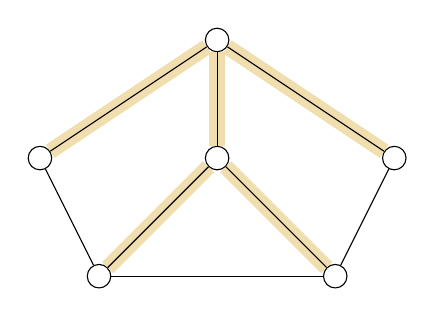
\begin{tikzpicture}[scale=0.75]
      \node[draw,circle, inner sep=3pt] (q) at (0,0)   {};
      \node[draw,circle, inner sep=3pt] (w) at (-3,-2) {};
      \node[draw,circle, inner sep=3pt] (e) at (0,-2)  {};
      \node[draw,circle, inner sep=3pt] (r) at (3,-2)  {};
      \node[draw,circle, inner sep=3pt] (t) at (-2,-4) {};
      \node[draw,circle, inner sep=3pt] (y) at (2,-4)  {};
      
      \draw[preaction={draw=darktan, line width=2mm}] (q) -- (w); 
      \draw[preaction={draw=darktan, line width=2mm}] (q) -- (e); 
      \draw[preaction={draw=darktan, line width=2mm}] (q) -- (r); 
      \draw (w) -- (t); 
      \draw[preaction={draw=darktan, line width=2mm}] (e) -- (t); 
      \draw[preaction={draw=darktan, line width=2mm}] (e) -- (y); 
      \draw (r) -- (y); 
      \draw (t) -- (y); 
    \end{tikzpicture}
  \end{minipage}
  \hspace{0.75cm}
  \begin{minipage}{.4\textwidth}
    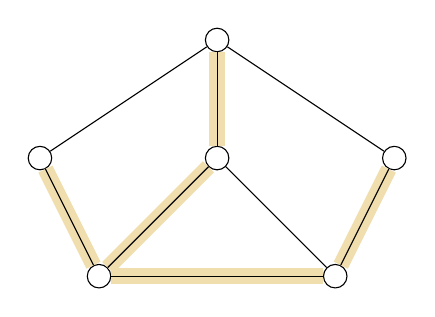
\begin{tikzpicture}[scale=0.75]
      \node[draw,circle, inner sep=3pt] (q) at (0,0)   {};
      \node[draw,circle, inner sep=3pt] (w) at (-3,-2) {};
      \node[draw,circle, inner sep=3pt] (e) at (0,-2)  {};
      \node[draw,circle, inner sep=3pt] (r) at (3,-2)  {};
      \node[draw,circle, inner sep=3pt] (t) at (-2,-4) {};
      \node[draw,circle, inner sep=3pt] (y) at (2,-4)  {};
      
      \draw (q) -- (w); 
      \draw[preaction={draw=darktan, line width=2mm}] (q) -- (e); 
      \draw (q) -- (r); 
      \draw[preaction={draw=darktan, line width=2mm}] (w) -- (t); 
      \draw[preaction={draw=darktan, line width=2mm}] (e) -- (t); 
      \draw (e) -- (y); 
      \draw[preaction={draw=darktan, line width=2mm}] (r) -- (y); 
      \draw[preaction={draw=darktan, line width=2mm}] (t) -- (y); 
    \end{tikzpicture}
  \end{minipage}

  \caption{Two spanning trees of a graph with 8 edges.}
  \label{fig:ex-graph-mst}
\end{figure}
  


\subsection{Other characterizations of a matroid} 
\label{sec:characterizations}

We have already seen the independent sets characterization of a matroid, but the other properties of a matroid have their own axiom systems that can equivalently be used to characterize a matroid.

\paragraph{Characterization via rank function.} \skelpar

\paragraph{Characterization via circuits.} A \textit{circuit} is a minimal dependent set of a matroid -- it is an independent set plus one redundant element. Equivalently, the collection of circuits of a matroid is given by
$$\mathcal{C} = \bigl\{ C : |C| = v(C) + 1, C\subseteq E \bigr\}.$$
A set is independent if and only if it contains no circuit~\cite{schrijver-2003}, and so a matroid is uniquely determined by the collection of its circuits. The following conditions characterize $\mathcal{C}$~\cite{whitney-1935}:
\begin{enumerate}
  \item[(1)] No proper subset of a circuit is a circuit.
  \item[(2)] If $C, C'\in\mathcal{C}$, $x\in C\cap C'$ and $y\in C\setminus C'$, then $C\cup C'$ contains a circuit containing $y$ but not $x$.
\end{enumerate}

\begin{figure}
  \centering
  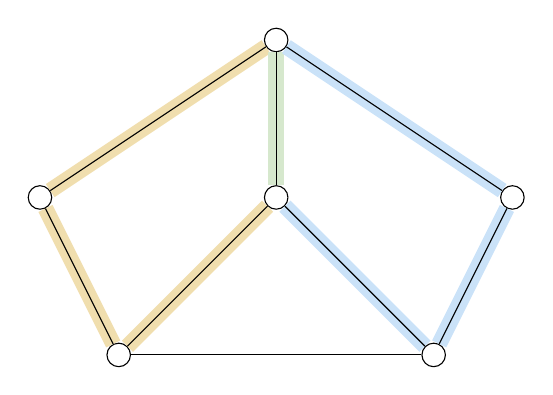
\begin{tikzpicture}
    \node[draw,circle, inner sep=3pt] (q) at (0,0)   {};
    \node[draw,circle, inner sep=3pt] (w) at (-3,-2) {};
    \node[draw,circle, inner sep=3pt] (e) at (0,-2)  {};
    \node[draw,circle, inner sep=3pt] (r) at (3,-2)  {};
    \node[draw,circle, inner sep=3pt] (t) at (-2,-4) {};
    \node[draw,circle, inner sep=3pt] (y) at (2,-4)  {};
    
    \draw[preaction={draw=darktan, line width=2mm}]           (q) -- (w); 
    \draw[preaction={draw=averagegreen, line width=2mm}]      (q) -- (e); 
    \draw[preaction={draw=complementaryblue, line width=2mm}] (q) -- (r); 
    \draw[preaction={draw=darktan, line width=2mm}] (w) -- (t); 
    \draw[preaction={draw=darktan, line width=2mm}] (e) -- (t); 
    \draw[preaction={draw=complementaryblue, line width=2mm}] (e) -- (y); 
    \draw[preaction={draw=complementaryblue, line width=2mm}] (r) -- (y); 
    \draw (t) -- (y); 
  \end{tikzpicture}
  \caption{Two overlapping circuits on a graph.}
  \label{fig:ex-graph-circuits}
\end{figure}

These properties are easily grokked by studying an example. In Figure~\ref{fig:ex-graph-circuits}, we see two circuits of a graph, highlighted in yellow and blue, overlapping at the edge highlighted in green. Obviously, no circuit in this figure contains a circuit. We can also verify that the union of the yellow edge set and the blue edge set, minus the green edge, is in fact a third, bigger circuit, as promised by property (2).

\paragraph{Characterization via closed sets.} We also need to establish the concept of the \textit{closed sets} (sometimes referred to as \textit{flats}~\cite{schrijver-2003}) of a matroid. A closed set is a set whose cardinality is maximal for its rank. Equivalently to the definition given above, we can define a matroid as $\mathfrak{M} = (E, \mathcal{F})$, where $\mathcal{F}$ is the set of closed sets of $\mathfrak{M}$, satisfying the following properties~\cite{knuth-1975}:

\begin{enumerate}
  \item The set of all elements is closed: $E \in \mathcal{F}$
  \item The intersection of two closed sets is a closed set: If $A,B \in \mathcal{F},$ then $A \cap B \in \mathcal{F}$
  \item If $A \in \mathcal{F}$ and $a,b \in E \setminus A,$ then $b$ is a member of all sets in $\mathcal{F}$ containing $A \cup \{a\}$ if and only if $a$ is a member of all sets in $\mathcal{F}$ containing $A \cup \{b\}$
\end{enumerate}

The \textit{closure function} is the function $\fn{cl} : 2^E \to 2^E$, such that $$\fn{cl}(S) = \bigl\{ x \in E : \fn{v}(S) = \fn{v}(S \cup \{x\}) \bigr\}.$$ That is to say, the closure function, when given a set $S \subseteq E$, returns the set of elements in $x \in E$ such that $x$ can be added to $S$ with no increase in rank. It returns the closed set of the same rank as $S$, that contains $S$. The \textit{nullity} of a subset $S$ is the difference $|S| - v(S)$, ie. the number of elements that must be removed from $S$ to obtain an independent set.

Figure~\ref{fig:ex-graph-closure} shows an independent (acyclic) set $S$ of edges in highlighted yellow, along with its closure $\fn{cl}(S)$ in blue. The closure is the set of edges $e$ such that $v(S+e) = v(S)$, or, equivalently, such that the spanning tree of $S+e$ has the same size as that of $S$.

\begin{figure}
  \centering
  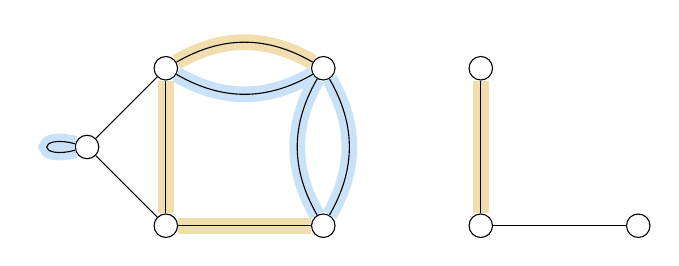
\begin{tikzpicture}[every loop/.style={}]
    \node[draw,circle,inner sep=3pt] (q) at (0,0) {};
    \node[draw,circle,inner sep=3pt] (w) at (2,0) {};
    \node[draw,circle,inner sep=3pt] (e) at (-1,-1) {};
    \node[draw,circle,inner sep=3pt] (r) at (0,-2) {};
    \node[draw,circle,inner sep=3pt] (t) at (2,-2) {};
    \node[draw,circle,inner sep=3pt] (y) at (4, 0) {};
    \node[draw,circle,inner sep=3pt] (u) at (4,-2) {};
    \node[draw,circle,inner sep=3pt] (i) at (6,-2) {};
    
    \begin{scope}[on background layer]
      \draw[line width=2mm, complementaryblue] (t) to [bend left] (w);
    \end{scope}
    
    \path (q) edge [bend left, preaction={draw=darktan, line width=2mm}] node {} (w);
    \path (q) edge [bend right, preaction={draw=complementaryblue, line width=2mm}] node {} (w);
    \draw (q) -- (e);
    \draw[preaction={draw=darktan, line width=2mm}] (q) -- (r);
    \path (e) edge [loop left, preaction={draw=complementaryblue, line width=2mm}] node {} (e);
    \draw (e) -- (r);
    \draw[preaction={draw=darktan, line width=2mm}] (r) -- (t);
    \path (t) edge [bend left] node {} (w);
    \path (t) edge [bend right, preaction={draw=complementaryblue, line width=2mm}] node {} (w);
    \draw[preaction={draw=darktan, line width=2mm}] (y) -- (u);
    \draw (u) -- (i);
  \end{tikzpicture}
  \caption{An independent subset of edges in yellow, with its closure in blue.}
  \label{fig:ex-graph-closure}
\end{figure}

\subsection{Matroid union}
\label{sec:matroid-union}
The matroid union is an operation that allows us to produce a new matroid by combining the independent sets of a collection of existing matroids. This is a powerful tool, as it allows us to reason about independence across multiple matroids, and has found several practical applications within fair allocation.

Given $n$ matroids $\mathfrak{M}_i = (E, \mathcal{I}_i)$, their union is given, somewhat obtusely, by $$\widehat{\mathfrak{M}} = (E, \widehat{\mathcal{I}}) = (E, \{ I_1\cup\ldots\cup I_n : I_i\in\mathcal{I}_i,\ \forall i\in N \}).$$ 
$\widehat{\mathfrak{M}}$ is in fact a matroid~\cite[Ch. 42]{schrijver-2003}, whose independent sets are the the subsets $S\subseteq E$ that allow an $n$-partition $S_1,\ldots,S_n$ such that $S_i\in\mathcal{I}_i$, for all $i\in N$. The following holds for all $n$-partitions of the elements of $E$:
$$S=(S_1,\dots,S_n)\in\mathcal{I}_i\times\dots\times\mathcal{I}_n 
\iff \bigcup_{i=1}^n S_i \in \widehat{\mathcal{I}}.$$

In fair allocation jargon, if each $\mathfrak{M}_i$ is the matroid described by agent $i$'s valuation function $v_i$, a set of goods $S$ is independent in $\widehat{\mathfrak{M}}$ if and only if we can allocate it among the agents and produce utilitarian social welfare (ie. total value) equal to $|S|$. This follows from the fact that if $\mathcal{S}$ is an $n$-partition of $S$ such that $\mathcal{S} = (S_1,\dots,S_n)\in\mathcal{I}_1\times\dots\times\mathcal{I}_n$, then $S_i\in\mathcal{I}_i$ for each $i$. When this is the case, we have $v_i(S_i) = |S_i|$, and so SW$(S) = \sum_{i\in N}v_i(S_i) = \sum_{i\in N}|S_i| = |S|$.

Hence, each basis in $\widehat{\mathfrak{M}}$ corresponds to a clean (but not necessarily complete), MAX-USW allocation of the goods in $E$~\cite{barman2021existence}. It is a classic result of Edmonds~\cite{Edmonds2009} that a basis in $\widehat{\mathfrak{M}}$ can be computed in polynomial time, using the \textit{matroid union algorithm}. This is achieved by making use of two additional concepts, the \textit{exchange graph} and \textit{transfer paths}. 

\subsubsection*{The exchange graph}
Given $n$ matroids $\mathfrak{M}_1 = (E, \mathcal{I}_1),\ldots,\mathfrak{M}_n = (E,\mathcal{I}_n)$, let $A$ be a collection of $n$ sets $A_1,\dots,A_n$ such that (a) $A_i\cap A_j = \emptyset$ when $i\neq j$, and (b) for each $i$, $A_i\subseteq E$ and $A_i\in\mathcal{I}_i$. In the context of a matroid-rank-valued fair allocation problem, $A$ is a clean allocation of the goods in $E$ to the agents in $N$.

We follow the example of Schrijver~\cite{schrijver-2003} and define the exchange graph of $A$ as the directed graph $D(A)=(E, x(A))$, where each node corresponds to a good in $E$, and the edges are given by
$$x(A) = \{ (p,q) : p \in A_i, q \in E\setminus A_i, v_i(A_i - p + q) = v_i(A_i) \},$$
where $v_i$ is the rank function of the matroid $\mathfrak{M}_i$. In other words, an edge exists between goods $p\in A_i$ and $q\in E\setminus A_i$ iff we can replace $p$ with $q$ for no decrease in the rank of the set containing $p$. Intuitively, we can understand $D$ as representing for each good $p$, which other good $q$ the current owner of $p$ can replace $p$ with and be just as happy. This intuitive explanation lets us begin to see why the matroid union algorithm and the concept of the exchange graph has found widespread use in fair allocation with matroid-rank valuations; they allow us to model equitable transfers of goods between agents.

\subsubsection*{Transfer paths and path augmentation}
Let $P = (e_1, \dots, e_t)$ be a path in the exchange graph $D(A)$. The \textit{transfer} of goods along $P$ is the operation in which $e_t$ is given to the agent who owns $e_{t-1}$, $e_{t-1}$ is given to the agent who owns $e_{t-2}$, and so on until $e_1$ is discarded. This transfer is called \textit{path augmentation}; we use the notation established by Viswanathan and Zick~\cite{viswanathan2023yankee} and denote the bundle $A_i$ after augmentation with the path $P$ by $A_i \Lambda P$. 

For some $i\in N$, we define $F_i = \{ e\in E\setminus A_i : A_i + e \in \mathcal{I}_i \}$ as the set of elements whose addition to $A_i$ yields another, larger independent set (remember that $A$ is clean, so $A_i\in\mathcal{I}_i$ for each $i$). In a paper on the matroid union algorithm, Knuth~\cite{knuth1973matroidpartitioning} shows that, by augmenting along a shortest path $P = (e_1,\dots,e_t)$ from $F_i$ to $A_j$ for some $j \in N - i$, we get
\begin{enumerate}
  \item[(a)] $v_i(A_i\Lambda P + e_1) = v_i(A_i) + 1$,
  \item[(b)] $v_k(A_k\Lambda P) = v_k(A_k),\ \forall k\in N - i - j$, and
  \item[(c)] $v_j(A_j\Lambda P) = v_j(A_j) - 1$.
\end{enumerate}
By greedily growing clean bundles in this manner, we can find a maximal independent set over $\widehat{\mathfrak{M}}$ in polynomial time~\cite{schrijver-2003}. Chapter~\ref{chap:matroids.jl} discusses Matroids.jl implementation of Knuth's matroid union algorithm. Viswanathan and Zick's Yankee Swap algorithm~\cite{viswanathan2023yankee}, discussed in Chapter~\ref{chap:yankee-swap}, uses these concepts as well.

\subsection{Matroid erection}
Knuth's general matroid construction, the implementation of which is discussed in Section~\ref{sec:kmc}, requires us to establish a few more matroid concepts. The \textit{rank-k truncation} of a rank-$r$ matroid $\mathfrak{M} = (E, \mathcal{I})$, is the rank-$k$ matroid $\mathfrak{M}^{(k)} = (E, \mathcal{I}^{(k)})$, where
$$\mathcal{I}^{(k)} = \{ I \in \mathcal{I} : |I| \leq k \}.$$
The \textit{truncation} of $\mathfrak{M}$ is given as $T(\mathfrak{M}) = \mathfrak{M}^{(r-1)}$. As a simple example, we have that the uniform matroid $U_n^{n-1} = T(F_n)$, where $F_n$ is the free matroid with $n$ elements. The \textit{erection} (I defer to Crapo for the somewhat esoteric choice of term~\cite{Crapo1970}) of the matroid $\mathfrak{M}$ is the matroid $\mathfrak{N}$ of rank $\leq r+1$ such that $\mathfrak{M} = T(\mathfrak{N})$. In other words, when taking the truncation of a matroid, we produce a new matroid by disregarding all independent sets of cardinality higher than some $k$. When taking the erection of a rank-$k$ matroid, we produce a new matroid by declaring some number of subsets $S \subseteq E$ such that $|S|=r+1$ to be independent, or equivalently, declaring some number of them to be closed sets of rank $r$. By declaring all of them to be dependent, we get the \textit{trivial erection} $\mathfrak{N} = \mathfrak{M}$. By declaring none of them dependent (ie. they are all independent sets $r(S) = |S| = r+1$), $\mathfrak{N}$ is the \textit{free erection} of $\mathfrak{M}$~\cite{greene-1991}.

\begin{figure}\centering
  \resizebox{\columnwidth}{!}{
         \begin{tikzpicture}[> = stealth,  shorten > = 1pt,   auto,   node distance = 1.5cm, mynode/.style={pattern=north east lines, circle, draw,inner sep=2pt,outer sep=0pt}]
  
  %%% LEVEL 1
  \node[draw, mynode]  (x) {1111};
  %%% LEVEL 2
  \node[draw, mynode]  [below left of=x] (B) {1101};
  \node[draw, mynode] [below right of=x]  (C) {1011};
  \node[draw, mynode]  [left  of=B] (A) {1110};
  \node[draw, mynode] [right of=C]  (D) {0111};
  %%%% LEVEL 3
  \node[draw, mynode, fill=darktan] [below of=B]  (AD) {0110};
  \node[draw, mynode, fill=darktan] [below of=C]  (BC) {1001};
  \node[draw, mynode, fill=darktan] [below of=D]  (BD) {0101};
  \node[draw, mynode, fill=darktan] [below of=A]  (AC) {1010};
  \node[draw, mynode, fill=darktan] [left  of=AC] (AB) {1100};
  \node[draw, mynode, fill=darktan] [right of=BD] (CD) {0011};
  
  %%  LEVEL   4
  \node[draw, mynode, fill=darktan] [below of=AD]  (ABD) {0100};
  \node[draw, mynode, fill=darktan] [below of=BC]  (ACD) {0010};
  \node[draw, mynode, fill=darktan] [left of=ABD]  (ABC) {1000};
  \node[draw, mynode, fill=darktan] [right of=ACD] (BCD) {0001};
  
  %%%% LEVEL 5
  \node[draw, mynode, fill=darktan] [below right of=ABD]  (ABCD) {0000};

  \begin{scope}[on background layer]
    \draw[line width=2mm, darktan] (AB) to (ABC);
    \draw[line width=2mm, darktan] (AB) to (ABD);
    \draw[line width=2mm, darktan] (AC) to (ABC);
    \draw[line width=2mm, darktan] (AC) to (ACD);
    \draw[line width=2mm, darktan] (AD) to (ABD);
    \draw[line width=2mm, darktan] (AD) to (ACD);
    \draw[line width=2mm, darktan] (BC) to (ABC);
    \draw[line width=2mm, darktan] (BC) to (BCD);
    \draw[line width=2mm, darktan] (BD) to (ABD);
    \draw[line width=2mm, darktan] (BD) to (BCD);
    \draw[line width=2mm, darktan] (CD) to (ACD);
    \draw[line width=2mm, darktan] (CD) to (BCD);
  \end{scope}
  
  
  %% LEVEL 1 to LEVEL 2
      \path (x)  edge node {} (A);
      \path (x)  edge node {} (B);
      \path (x)  edge node {} (C);
      \path (x)  edge node {} (D);
  
  %% LEVEL 2 to LEVEL 3
      \path (A)  edge node {} (AB);
      \path (A)  edge node {} (AC);
      \path (A)  edge node {} (AD);
      \path (B)  edge node {} (AB);
      \path (B)  edge node {} (BC);
      \path (B)  edge node {} (BD);
      \path (C)  edge node {} (AC);%
      \path (C)  edge node {} (BC);
      \path (C)  edge node {} (CD);
      \path (D)  edge node {} (AD);
      \path (D)  edge node {} (BD);
      \path (D)  edge node {} (CD);
  %%% LEVEL 3 TO 4
  
      \path (AB)  edge node {} (ABC);
      \path (AB)  edge node {} (ABD);
      \path (AC)  edge node {} (ABC);
      \path (AC)  edge node {} (ACD);
      \path (AD)  edge node {} (ABD);
      \path (AD)  edge node {} (ACD);
      \path (BC)  edge node {} (ABC);
      \path (BC)  edge node {} (BCD);
      \path (BD)  edge node {} (ABD);
      \path (BD)  edge node {} (BCD);
      \path (CD)  edge node {} (ACD);
      \path (CD)  edge node {} (BCD);
  %%%% LEVEL 4 to 5
      \path (ABC)  edge [preaction={draw=darktan, line width=2mm}] node {} (ABCD);
      \path (ABD)  edge [preaction={draw=darktan, line width=2mm}] node {} (ABCD);
      \path (ACD)  edge [preaction={draw=darktan, line width=2mm}] node {} (ABCD);
      \path (BCD)  edge [preaction={draw=darktan, line width=2mm}] node {} (ABCD);

      %%%% Dashed lines
% \draw[dashed] (-6,-0.5) -- (6,-0.5); 
% \node[] at (-6,0) {Rank 4};
% \draw[dashed] (-6,-1.75) -- (6,-1.75); 
% \node[] at (-6,-1) {Rank 3};
\draw[dashed] (-6,-3.5) -- (6,-3.5); 
\node[] at (-6,-2.625) {Rank 2};
\draw[dashed] (-6,-4.625) -- (6,-4.625); 
\node[] at (-6,-4) {Rank 1};
\node[] at (-6,-5) {Rank 0};

        \end{tikzpicture}
  }
  \caption{The uniform matroid $U_4^2$.}
  \label{fig:hasse-uniform}
\end{figure}

\begin{figure}\centering
  \resizebox{\columnwidth}{!}{
         \begin{tikzpicture}[> = stealth,  shorten > = 1pt,   auto,   node distance = 1.5cm, mynode/.style={pattern=north east lines, circle, draw,inner sep=2pt,outer sep=0pt}]
  
  %%% LEVEL 1
  \node[draw, mynode]  (x) {1111};
  %%% LEVEL 2
  \node[draw, mynode, fill=darktan]  [below left of=x] (B) {1101};
  \node[draw, mynode, fill=darktan] [below right of=x]  (C) {1011};
  \node[draw, mynode, fill=darktan]  [left  of=B] (A) {1110};
  \node[draw, mynode] [right of=C]  (D) {0111};
  %%%% LEVEL 3
  \node[draw, mynode, fill=darktan] [below of=B]  (AD) {0110};
  \node[draw, mynode, fill=darktan] [below of=C]  (BC) {1001};
  \node[draw, mynode, fill=darktan] [below of=D]  (BD) {0101};
  \node[draw, mynode, fill=darktan] [below of=A]  (AC) {1010};
  \node[draw, mynode, fill=darktan] [left  of=AC] (AB) {1100};
  \node[draw, mynode, fill=darktan] [right of=BD] (CD) {0011};
  
  %%  LEVEL   4
  \node[draw, mynode, fill=darktan] [below of=AD]  (ABD) {0100};
  \node[draw, mynode, fill=darktan] [below of=BC]  (ACD) {0010};
  \node[draw, mynode, fill=darktan] [left of=ABD]  (ABC) {1000};
  \node[draw, mynode, fill=darktan] [right of=ACD] (BCD) {0001};
  
  %%%% LEVEL 5
  \node[draw, mynode, fill=darktan] [below right of=ABD]  (ABCD) {0000};

  \begin{scope}[on background layer]
    \draw[line width=2mm, darktan] (A) to (AB);
    \draw[line width=2mm, darktan] (A) to (AC);
    \draw[line width=2mm, darktan] (A) to (AD);
    \draw[line width=2mm, darktan] (B) to (AB);
    \draw[line width=2mm, darktan] (B) to (BC);
    \draw[line width=2mm, darktan] (B) to (BD);
    \draw[line width=2mm, darktan] (C) to (AC);
    \draw[line width=2mm, darktan] (C) to (BC);
    \draw[line width=2mm, darktan] (C) to (CD);
    
    \draw[line width=2mm, darktan] (AB) to (ABC);
    \draw[line width=2mm, darktan] (AB) to (ABD);
    \draw[line width=2mm, darktan] (AC) to (ABC);
    \draw[line width=2mm, darktan] (AC) to (ACD);
    \draw[line width=2mm, darktan] (AD) to (ABD);
    \draw[line width=2mm, darktan] (AD) to (ACD);
    \draw[line width=2mm, darktan] (BC) to (ABC);
    \draw[line width=2mm, darktan] (BC) to (BCD);
    \draw[line width=2mm, darktan] (BD) to (ABD);
    \draw[line width=2mm, darktan] (BD) to (BCD);
    \draw[line width=2mm, darktan] (CD) to (ACD);
    \draw[line width=2mm, darktan] (CD) to (BCD);
  \end{scope}
  
  
  %% LEVEL 1 to LEVEL 2
      \path (x)  edge node {} (A);
      \path (x)  edge node {} (B);
      \path (x)  edge node {} (C);
      \path (x)  edge node {} (D);
  
  %% LEVEL 2 to LEVEL 3
      \path (A)  edge node {} (AB);
      \path (A)  edge node {} (AC);
      \path (A)  edge node {} (AD);
      \path (B)  edge node {} (AB);
      \path (B)  edge node {} (BC);
      \path (B)  edge node {} (BD);
      \path (C)  edge node {} (AC);%
      \path (C)  edge node {} (BC);
      \path (C)  edge node {} (CD);
      \path (D)  edge node {} (AD);
      \path (D)  edge node {} (BD);
      \path (D)  edge node {} (CD);
  %%% LEVEL 3 TO 4
  
      \path (AB)  edge node {} (ABC);
      \path (AB)  edge node {} (ABD);
      \path (AC)  edge node {} (ABC);
      \path (AC)  edge node {} (ACD);
      \path (AD)  edge node {} (ABD);
      \path (AD)  edge node {} (ACD);
      \path (BC)  edge node {} (ABC);
      \path (BC)  edge node {} (BCD);
      \path (BD)  edge node {} (ABD);
      \path (BD)  edge node {} (BCD);
      \path (CD)  edge node {} (ACD);
      \path (CD)  edge node {} (BCD);
  %%%% LEVEL 4 to 5
      \path (ABC)  edge [preaction={draw=darktan, line width=2mm}] node {} (ABCD);
      \path (ABD)  edge [preaction={draw=darktan, line width=2mm}] node {} (ABCD);
      \path (ACD)  edge [preaction={draw=darktan, line width=2mm}] node {} (ABCD);
      \path (BCD)  edge [preaction={draw=darktan, line width=2mm}] node {} (ABCD);
      
      %%%% Dashed lines
% \draw[dashed] (-6,-0.5) -- (6,-0.5); 
% \node[] at (-6,0) {Rank 4};
\draw[dashed] (-6,-1.75) -- (1.75,-1.75); 
\draw[dashed] (1.75,-1.75) -- (1.75,-0.25); 
\draw[dashed] (1.75,-0.25) -- (6,-0.25); 
\node[] at (-6,-1) {Rank 3};
\draw[dashed] (-6,-3.5) -- (6,-3.5); 
\node[] at (-6,-2.625) {Rank 2};
\draw[dashed] (-6,-4.625) -- (6,-4.625); 
\node[] at (-6,-4) {Rank 1};
\node[] at (-6,-5) {Rank 0};

        \end{tikzpicture}
  }
  \caption{An erection of $U_4^2$.}
  \label{fig:hasse-erection}
\end{figure}

A matroid can have many erections. Figure~\ref{fig:hasse-uniform} shows the Hasse diagram for the matroid of 4 elements, where every subset of two or fewer elements is independent (denoted in yellow). Each subset is encoded as a binary string, where a 1 designates membership in the set (a syntax we will become very familiar with in Chapter~\ref{chap:generating_matroids}). This matroid is known as the uniform matroid $U_4^2$. The uniform matroid $U_4^3$ is the free erection of $U_4^2$, where we have simply designated all sets of rank 3 as independent. Figure~\ref{fig:hasse-erection} shows another erection of $U_4^2$, one in which only three of the subsets with three elements are designated as independent. The final set, 0111, remains a dependent set, and has therefore in fact been designated as a closed set of rank $2$. By starting from the rank-0 matroid $\mathfrak{M}^{(0)}$, one can iteratively erect any matroid $\mathfrak{M}$, at each iteration $i$ designating the sets to be closed sets of rank $i$ (all the while ensuring that the axioms for the closed sets of a matroid are obeyed). This is the approach taken by Knuth in his matroid erection algorithm, which is discussed in Chapter~\ref{sec:kmc}.



\section{Matroids in fair allocation}
It should be clear at this point that matroids are compelling structures to work with in the context of fair allocations. There are two main use cases for matroids in fair allocation: matroid-rank valuation functions (as in the example scenario from the introduction) and matroid constraints. Matroids.jl will be developed with the empirical study of algorithms for these two scenarios in mind.

\subsection{Matroid-rank valuations}
In a fair allocation instance with matroid-rank valuations, each agent $i$ has a corresponding matroid $\mathfrak{M}_i = (\mathcal{M}, \mathcal{I}_i)$, where $\mathcal{M}$ (the set of goods) is the ground set of elements common to all agents' matroids.

Babaioff 2021 -- PE mechanism -- non-redundant Lorenz dominating allocation always exists and is MNW, MAX-USW, leximin, EFX (EF1) and .5-MMS. With a randomized prioritization it is ex ante EF and ex ante proportional as well. 3Yankee Swap computes prioritized non-redundant Lorenz dominating allocations.


Limitation: MRFs cannot model complementary goods!


\subsection{Matroid constraints}
Another usage found for matroids in fair allocation is that of \textit{matroid constraints}. The majority of work on fair division assumes that any allocation is feasible, and the sole concern is finding an allocation that aligns well with the agents' valuation profiles. In many practical applications, however, there will be allocations that are not legal or desirable. Suksompong~\cite{suksumpong-constraints} gives the example of a museum with multiple branches distributing exhibits of different categories (sculpture, paintings, et cetera) among the branches. For each category, it wants to create a balanced distribution among the branches, so that the difference in the number of exhibits of a given category differ by at most one between any branch. This is an example of a \textit{cardinality constraint}, which can be modeled with a partition matroid, and is a subset of the broader class of matroid constraints. 

When matroid constraints are enforced on a fair allocation instance, we require that all bundles be independent sets on some supplied matroid, common to all agents. 
\chapter{The Matroids.jl API}
\label{chap:matroids.jl}
Matroids.jl exists to enable the empirical study of matroidal fair allocation. In this chapter, I consider what fair allocation-specific methods the Matroids.jl API should expose to achieve this goal, and how they might be implemented. While doing so, I keep track of which properties are required from the matroids being used. Chapter~\ref{chap:generating_matroids} describes how Matroids.jl generates a number of different matroid types, and how the getter functions for the properties we need are implemented.

The implementation will draw inspiration from, and be designed to integrate with, Hummel and Hetland's well-organized Allocations.jl library~\cite{Hetland_Allocations_jl_2022}, which provides a range of algorithms for fair allocation of indivisible items. Allocations.jl currently supports additive and submodular valuations and a number of constraint types, including conflict constraints and cardinality constraints. Matroids.jl should extend Allocations.jl with support for matroid-rank valuations and matroidal constraints. As such, Matroids.jl should be structured in such a manner as to be familiar to those acquainted with Allocations.jl.

In this chapter, I describe how the Matroids.jl API is designed to enable experimentation with fair allocation algorithms for matroid-rank valuations. First, I describe how Matroids.jl extends the fairness and efficiency measures of Allocations.jl to handle matroid-rank valuations. With that in hand, I enumerate a few recent, interesting algorithms for this use case, and discuss which requirements their implementation would pose to Matroids.jl. Finally, I show how Matroids.jl supports the matroid union operation, using a classic matroid procedure attributable to Knuth~\cite{knuth1973matroidpartitioning} and Edmonds~\cite{Edmonds2009} that have found widespread use in fair allocation with matroid-rank valuations.

Implementing support for matroidal constraints is out of scope for this thesis. A discussion on how one might go about doing this in the future is included in Chapter~\ref{chap:conclusions}.

\section{Fairness under matroid-rank valuations}
If Matroids.jl is to be of use in the empirical study of matroidal fair allocation algorithms, we need to be able to evaluate the fairness of an allocation. In this chapter, I show how Matroids.jl implements the fairness criteria given in Chapter~\ref{chap:prelims}. The valuation profile of matroid-rank-valued allocation problem instance gives the valuation function of each agent. This is represented as a struct containing the matroid $\mathfrak{M}_i$ for each agent $i$. Agent $i$'s value for the set of goods $S$, $v_i(S)$, is the rank of $S$ in $\mathfrak{M}_i$.
\begin{figure}[ht!]
\begin{jllisting}
"""
    struct MatroidRank <: Profile

A matroid rank valuation profile, representing how each agent values all possible bundles. The profile is constructed from `n` matroids, one for each agents, each matroid over the set of goods {1, ..., m}. 
"""
struct MatroidRank <: Profile
    Ms::Vector{Matroid}
    m::Int
end

value(V::MatroidRank, i, S) = rank(V.Ms[i], S)
value(V::MatroidRank, i, g::Int) = value(V, i, Set(g))
\end{jllisting}
\caption{\jlinl{MatroidRank} represents a fair allocation instance with matroid-rank valuations.}
\end{figure}

\subsection*{Envy-freeness}
Checking if an allocation is EF is the same for matroid-rank valuations as for additive valuations -- simply compare each agent's own bundle value with that agent's subjective valuation of each other agent's bundle. This is already implemented in Allocations.jl. In this section, I give the functions \jlinl{value_1}, \jlinl{value_x} and \jlinl{value_x0}, which are used for computing EF1, EFX$_+$ and EFX$_0$, respectively. These functions take in a valuation profile, an agent $i$ and a bundle $S$, and return the agent $i$'s value for $S$, up to some item. 

To check efficiently if an allocation is EF1, we make use of the fact that a matroid rank function has binary marginals; in other words, the highest valued good in a bundle will always have value 1, unless the bundle value is 0. This gives us a simple way of checking for EF1. Similarly, since the least positively-valued good also has value 1, EFX$_+$ is the same as EF1.
\begin{figure}[ht!]
\begin{jllisting}
value_1(V::MatroidRank, i, S) = max(value(V, i, S) - 1, 0)
value_x(V::MatroidRank, i, S) = value_1(V, i, S)
value_x0(V::MatroidRank, i, A) =
    is_indep(V.Ms[i], A) ? value_1(V, i, A) : value(V, i, A)
\end{jllisting}
\caption{Methods for computing EF1, EFX$_+$ and EFX$_0$.}
\end{figure}

The value of the least valued good overall (including 0-values) depend on whether the bundle is independent. An independent set contains by definition no redundant elements, so if the bundle is independent, the least-valued good has value 1. If the bundle is dependent, it contains at least one 0-valued good, or, equivalently, a good whose removal does not affect the bundle value. This gives us EFX$_0$.

\subsection*{Proportionality}
To check whether an allocation $A$ is PROP or some relaxation thereof, we compare $v_i(A_i)$ against some threshold for every agent $i$. In this section, we give the functions for computing the threshold for PROP and its relaxations.

\begin{figure}[ht!]
\begin{jllisting}
prop(V::MatroidRank, i, _) = rank(V.Ms[i])/na(V)
prop_1(V::MatroidRank, i, A) = prop(V, i, A) - 1
prop_x(V::MatroidRank, i, A) = prop_1(V, i, A)
prop_x(V::MatroidRank, i, A) = 
    is_closed(V.Ms[i], A) ? prop_1(V, i, A) : prop(V, i, A)
\end{jllisting}
\caption{Methods for computing PROP, PROP1, PROPX$_+$ and PROPX$_0$.}
\end{figure}

PROP$_i$ is simply the rank of $\mathfrak{M}_i$, $v_i(\mathcal{M})$, as this is the maximum value achievable for agent $i$, divided by the number of agents in the problem instance.

To check for PROP1, we need to figure out if there exists some $g\in\mathcal{M}$ such that $v_i(A_i+g)\geq \frac{1}{n}v_i(\mathcal{M})$. We know, due to the hereditary property (as given in Section~\ref{sec:characterizations}) that unless $v_i(A_i) = v_i(\mathcal{M})$ already (in which case we have trivial PROP1), there exists $g\in\mathcal{M}\setminus A_i$ such that $\Delta_i(A_i, g) = 1$. To figure out if $A$ is PROP1, then, we need to check whether $v_i(A_i) + 1 \geq \frac{1}{n}v_i(\mathcal{M})$, or equivalently, whether $v_i(A_i) \geq \frac{1}{n}v_i(\mathcal{M})-1 = \text{PROP}_i - 1$. This is our PROP1 threshold. Since the least positively-valued element will also have a marginal value of 1, PROPX$_+$ is the same as PROP1.

When checking for PROPX$_0$, we want the $g\in E\setminus A_i$ whose addition would increase the value of $A_i$ the least. The question, then, is whether there exists an element $g\in E\setminus A_i$ such that $\Delta_i(A_i, g) = 0$. If $A_i$ is a closed set (ie. maximal for its rank), then any additional good will increase the rank by 1, otherwise there exists some such $g$.

\subsubsection*{Maximin share}
Matroids.jl implements Barman and Verma's~\cite[Appendix A]{barman2021existence} method for computing agent $i$'s maximin share in polynomial time. Recall that the maximin share for agent $i$,  $\mu_i$, is the best bundle value she can achieve by allocating the goods to the $n$ agents and choosing the worst bundle for herself. Barman and Verma show that even if we require each bundle considered to be clean (ie. independent in $\mathfrak{M}_i$), we still find $\mu_i$. The task, therefore, is to find the partition of $E$ into $n$ sets independent in $\mathfrak{M}_i$ maximizing the minimum bundle value.

This is equivalent to finding a maximum-size independent set in the $n$-fold union of $\mathfrak{M}_i$ with itself, ie.
$$\widehat{\mathfrak{M}}_{i \times n} = (E, \widehat{\mathcal{I}}_{i\times n}) = (E, \{ I_1\cup\dots\cup I_n : I_t \in \mathcal{I}_i,\ \forall t \in N \}),$$ 
which can be produced in polynomial time using the matroid union algorithm~\cite[Ch. 42]{schrijver-2003}. Let $\widehat{A}\in\widehat{\mathcal{I}}_{i\times n}$ be such a set. As shown in Section~\ref{sec:matroid-union}, $\widehat{A}$ allows an $n$-partition $A = (A_1,\dots,A_n)$ such that, in this case, $A_t\in\mathcal{I}_i$ for all $t\in N$.

\begin{figure}
    \begin{jllisting}
"""
    function mms_i(V, i)

Finds the maximin share of agent i in the instance V.
"""
function mms_i(V::MatroidRank, i)
    M_i = V.Ms[i]; n = na(V)

    # An initial partition into independent subsets (subjectively so for i).
    (A, _) = matroid_partition_knuth73([M_i for _ in 1:n])

    # Setup matrix D st D[j,k] v_i(A_j) - v_i(A_k) ∀ j,k ∈ [n].
    D = zeros(Int8, n, n)
    for j in 1:n, k in 1:n
        # v_i(A_p) = |A_p| since all sets in A are independent wrt M_i.
        D[j,k] = length(A[j]) - length(A[k])
    end

    jk = argmax(D)
    while D[jk] > 1
        j,k = Tuple(jk)

        # By the augmentation property, ∃g ∈ A_j st A_k + g ∈ I_i.
        g = nothing
        for h ∈ setdiff(A[j], A[k]) 
            if is_indep(M_i, A[k] ∪ h)
                g = h; break
            end 
        end

        # Update A.
        setdiff!(A[j], g); union!(A[k], g)

        # Update D.
        for l in 1:n
            D[j, l] -= 1; D[l, j] += 1 # A_j is one smaller.
            D[k, l] += 1; D[l, k] -= 1 # A_k is one larger.
        end

        jk = argmax(D)
    end
    
    return minimum(length, A)
end
    \end{jllisting}
    \caption{Maximin share computation.}
    \label{code:mms_i}
\end{figure}

Matroids.jl implements Knuth's 1973 matroid union algorithm~\cite{knuth1973matroidpartitioning}. This is detailed in Section~\ref{sec:matroid-union}, for now let it suffice to say that we have a function called\linebreak\jlinl{matroid_partition_knuth73}, which, when given $k$ matroids $(\mathfrak{M}_1,\dots,\mathfrak{M}_k)$ over the same ground set $E$, returns a partition of $E$ into $k$ sets $S = (S_1, \dots, S_k)$ such that each set $S_t$ is independent in $\mathfrak{M}_t$. By passing $n$ copies of $\mathfrak{M}_i$, we get the $n$-partition $A$ as above.

With $A$ in hand, Barman and Verma's procedure iteratively update the sets of $A$ as long as there exist $j, k \in N$ such that $v_i(A_j) - v_i(A_k) \geq 2$. This is equivalent to $|A_j| - |A_k| \geq 2$, since the sets are all independent in $\mathfrak{M}_i$. When this is the case, there exists (due to the exchange property) a good $g'\in A_j$ such that $A_k + g' \in \mathcal{I}_i$. The sets are updated $A_j \leftarrow A_j - g'$ and $A_k \leftarrow A_k + g'$ until no two sets differ in cardinality by more than one. Now, we have a partition of $E$ into $n$ evenly sized subsets that are independent in $\mathfrak{M}_i$. The value of worst of these is agent $i$'s maximin share. Matroids.jl's implementation of this procedure is given in Figure~\ref{code:mms_i}.




\section{Requirements of three selected algorithms}
The purpose of Matroids.jl being to enable the empirical study of matroidal fair allocation, we should investigate what requirements algorithms in this space pose of a library that purports to enable their implementation. In order to maintain a manageable scope for this thesis, I restrict my attention to three recent algorithms for fair allocation with matroid-rank valuations, that, while relatively short and sweet, make use of some deep results from matroid theory to deliver well on a range of fairness criteria.

\paragraph{The Envy-Induced Transfers algorithm.} This algorithm is due to Benabbou, Chakraborty, Igarashi and Zick~\cite{benabbou-2021}. Named Algorithm 1 in the paper, it relies on a subroutine the authors name \textit{Envy-Induced Transfers} (EIT)---hence the name. Benabbou et al show that, for matroid-rank valuations, a Pareto Optimal, MAX-USW and EF1 allocation always exist and can be computed efficiently, using the simple greedy algorithm given in Algorithm~\ref{alg:eit}.

The algorithm should look familiar; it is very similar to Barman and Verma's procedure for computing an agent's maximin share detailed in the previous section. The crux of both approaches is the concept of the matroid union: a maximum-size independent set in the union of the matroids in play is a clean MAX-USW allocation. With that in hand, we can use the exchange property of independent sets to greedily choose goods to transfer until the allocation has the desired properties. In this case, the algorithm continues transfering as long some agent envies another agent for more than one good; when it terminates, the allocation is thus EF1.

\begin{algorithm}{\pr{Envy-Induced-Transfers}~\cite{benabbou-2021}}{eit}

\begin{pseudo}[label=\small\arabic*, indent-mark]
    Compute a clean, MAX-USW allocation $A = (A_1,\dots,A_n)$ \\
    \kw{while} there are two agents $i,j\in N$ st. $i$ envies $j$ more than 1 good, \kw{do}  \\+
        Find good $g \in A_j$ with $\Delta_i(A_i, g) = 1$ \\
        Update $A_j \leftarrow A_j - g$ \\
        Update $A_i \leftarrow A_i + g$ \\-
    \kw{end}
    \kw{return} $A$
\end{pseudo}
  
  \end{algorithm}


\paragraph{AlgMMS.} This algorithm is given in Algorithm~\ref{alg:mms}, and is due to Barman and Verma~\cite{barman2021existence}. It is similar to \pr{Envy-Induced-Transfers} in that it first generates an initial clean, MAX-USW allocation using the matroid union algorithm, and then massages this allocation until some desired properties are met. In this case, the desired property is that of MMS-fairness; each agent should receive at least their share $\mu_i$, which is computed using the procedure described in the previous section.

\pr{AlgMMS} achieves this by keeping track of which agents have received more than their MMS (these make up the set $S_>$), and which have received less ($S_<$). While there are agents $i$ such that $v_i(A_i) < \mu_i$, the algorithm augments the allocation along a transfer path from a good for which $i$ has positive marginal value (the set of goods $F_i$), to a good currently located in $A_j$, for some $j\in S_>$. Barman and Verma show that this algorithm yields MMS-fair MAX-USW allocations. To build an intuitive understanding of why, let us take a look at an instructive example.

\pr{Envy-Induced-Transfers} can eliminate the envy one good at a time by moving a good directly from the envied to the envious agent. This is equivalent to augmenting along a length-1 transfer path on the exchange graph. \pr{AlgMMS}, on the other hand, might encounter a situation in which some agent has more than their MMS, whilst another has less, yet no good in the fortunate agent's bundle will improve the situation of the unfortunate one---in that case, there must be a transfer path of length > 1 between the two agents. Figure~\ref{fig:not_mms}~(a)-(c) illustrates such a situation.

\begin{figure}[ht!]
  \begin{subfigure}{0.3\textwidth}
    \centering
    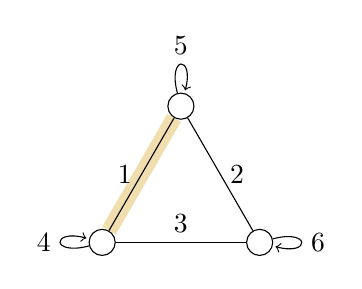
\begin{tikzpicture}
        \node[circle, draw] (1) at (0,0) {};
        \node[circle, draw] (2) at (2,0) {};
        \node[circle, draw] (3) at (1,1.73) {};
        
        \draw (1) --               node[above] {3} (2);
        \draw (2) --               node[right] {2} (3);
        \draw[preaction={draw=darktan, line width=2mm}] 
              (3) --               node[left]  {1} (1);
        \draw (1) edge[loop left]  node        {4} (1);
        \draw (2) edge[loop right] node        {6} (2);
        \draw (3) edge[loop above] node        {5} (3);
    \end{tikzpicture}
    \caption{Agent $a_1$}
  \end{subfigure}
  \hfill
  \begin{subfigure}{0.3\textwidth}
    \centering
    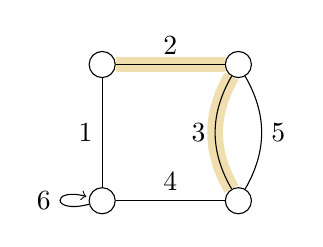
\begin{tikzpicture}
        \node[draw,circle] (r) at (0,0) {};
        \node[draw,circle] (q) at (0,1.73) {};
        \node[draw,circle] (w) at (1.73,1.73) {};
        \node[draw,circle] (t) at (1.73,0) {};

        \draw[preaction={draw=darktan, line width=2mm}] 
        (q) -- node[above] {2} (w);
        \draw
        (q) -- node[left] {1} (r);
        \draw
        (r) -- node[above] {4} (t);
        \path (t) 
        edge [bend left, preaction={draw=darktan, line width=2mm}] 
        node[left] {3} (w);
        \path (t) 
        edge [bend right]
        node[right] {5} (w);
        \path (r) 
        edge [loop left] 
        node[left] {6} (r);
    \end{tikzpicture}
    \caption{Agent $a_2$}
  \end{subfigure}
  \hfill
  \begin{subfigure}{0.3\textwidth}
    \centering
    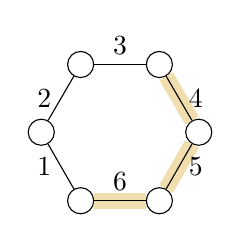
\begin{tikzpicture}        
        \node[draw, circle] (q) at (0,0)       {};
        \node[draw, circle] (w) at (1,0)       {};
        \node[draw, circle] (e) at (1.5,0.87)  {};
        \node[draw, circle] (r) at (1,1.73)    {};
        \node[draw, circle] (t) at (0,1.73)    {};
        \node[draw, circle] (y) at (-0.5,0.87) {};

        % Draw the edges
        \draw[preaction={draw=darktan, line width=2mm}] 
              (q) -- node[above] {6} (w);
        \draw[preaction={draw=darktan, line width=2mm}] 
              (w) -- node[right] {5} (e);
        \draw[preaction={draw=darktan, line width=2mm}] 
              (e) -- node[right] {4} (r);
        \draw (r) -- node[above] {3} (t);
        \draw (t) -- node[left]  {2} (y);
        \draw (y) -- node[left]  {1} (q);
    \end{tikzpicture}
    \caption{Agent $a_3$}
  \end{subfigure}

  \bigskip

  \begin{subfigure}{\textwidth}
    \centering
    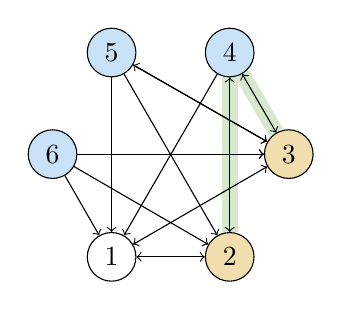
\begin{tikzpicture}[scale=1.5]
        \node[draw, circle]                         (1) at (0,0)       {1};
        \node[draw, circle, fill=darktan]           (2) at (1,0)       {2};
        \node[draw, circle, fill=darktan]           (3) at (1.5,0.87)  {3};
        \node[draw, circle, fill=complementaryblue] (4) at (1,1.73)    {4};
        \node[draw, circle, fill=complementaryblue] (5) at (0,1.73)    {5};
        \node[draw, circle, fill=complementaryblue] (6) at (-0.5,0.87) {6};

        \begin{scope}[on background layer]
            \draw[line width=2mm, averagegreen] (2) to (4);
            \draw[line width=2mm, averagegreen] (3) to (4);
        \end{scope}

        \draw[<->] (1) -- (2);
        \draw[<->] (1) -- (3);
        \draw[<-]  (1) -- (4);
        \draw[<->] (2) -- (4);
        \draw[<->] (3) -- (4);
        \draw[<->] (3) -- (5);
        \draw[->]  (5) -- (1);
        \draw[->]  (5) -- (2);
        \draw[->]  (5) -- (3);
        \draw[->]  (6) -- (1);
        \draw[->]  (6) -- (2);
        \draw[->]  (6) -- (3);
        \draw[->]  (6) -- (3);
    \end{tikzpicture}
    \caption{The exchange graph of the allocation}
  \end{subfigure}
  \caption{(a)-(c) shows three agents represented by their valuation matroids, the allocation $A$ highlighted in yellow. (d) shows the exchange graph $D(A)$, with $F_{a_1}$ highlighted in yellow, $S_>$ in blue and the transfer paths in green.}
  \label{fig:not_mms}
\end{figure}

\begin{algorithm}{\pr{AlgMMS}~\cite{barman2021existence}}{mms}
\begin{pseudo}[label=\small\arabic*, indent-mark]
Compute a clean, MAX-USW allocation $A = (A_1,\dots,A_n)$ \\
Initialize $S_< := \{ i\in N : v_i(A_i) < \mu_i \}$ \\
Initialize $S_> := \{ i\in N : v_i(A_i) > \mu_i \}$ \\
\kw{while} $S_<\neq\emptyset$, \kw{do}  \\+
    Select any agent $i \in S_<$\\
    Construct the exchange graph $D(A)$ \\
    Let $F_i := \{ g\in E : \Delta_i(A_i, g) = 1 \}$ \\
    Let $P = (g_1,\dots,g_t)$ be a shortest path $F_i \to \bigcup_{j\in S_>}A_j$ in $D(A)$ \\
    Update $A_k \leftarrow A_k\Lambda P$ for all $k\in N$ \\
    Update $A_i \leftarrow A_i + g_1$ and $A_j \leftarrow A_j - g_t$ \\
    Reset $S_< := \{ i\in N : v_i(A_i) < \mu_i \}$ \\
    Reset $S_> := \{ i\in N : v_i(A_i) > \mu_i \}$ \\-
\kw{end} \\
Let $junk := E \setminus \bigcup_{i=1}^n A_i$ be the set of unallocated goods \\
\kw{return} $(A_1 \cup junk, A_2,\dots,A_n)$
\end{pseudo}
  
\end{algorithm}

In this scenario, we have three agents $a_1, a_2$ and $a_3$ and six goods $E=\{1,\dots,6\}$. The allocation $A$ is highlighted in yellow: $A_{a_1} = \{1\}$, $A_{a_2} = \{2,3\}$ and $A_{a_3} = \{4,5,6\}$. It should be clear that the maximin share of each agent is 2; in the situation depicted, $a_3$ has received a bundle of value 3, at the expense of $a_1$, who only received a bundle of value 1. This might be the initial allocation produced with the matroid union algorithm (it is MAX-USW, as SW$(A) = 6 = |E|$). Since $v_{a_1}(A_{a_1}) = 1 < \mu_{a_1} = 2$, we have $S_<=\{a_1\}$, and need to transfer a good into $A_{a_1}$. However, since none of the goods in $A_{a_3}$ are of value to $a_1$, we need to find a transfer path via some other good.

Figure~\ref{fig:not_mms}(d) shows the exchange graph $D(A)$ (ie. the directed graph with a node per good, and an edge $(u,v)$ iff good $u$ can be exchanged with good $v$ for no loss in value for the current holder of $u$). Highlighted in yellow are the goods in $F_{a_1}$, the set of goods $g$ such that $\Delta_{a_1}(A_{a_1}, g) = 1$. The blue nodes are the goods belonging to an agent in $S_>$, the set of agents who have received more than their MMS. The green edges show the paths between these two sets of goods. As we can see, the available transfer paths are $(2,4)$ and $(3,4)$, representing a transfer of good 4 from $A_{a_3}$ to $A_{a_2}$, and good 2 or 3 from $A_{a_2}$ to $A_{a_1}$, respectively.

\begin{figure}[ht!]
    \begin{subfigure}{0.3\textwidth}
      \centering
      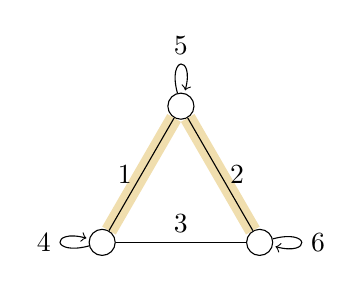
\begin{tikzpicture}
          \node[circle, draw] (1) at (0,0) {};
          \node[circle, draw] (2) at (2,0) {};
          \node[circle, draw] (3) at (1,1.73) {};
          
          \draw (1) --               node[above] {3} (2);
          \draw[preaction={draw=darktan, line width=2mm}]
                (2) --               node[right] {2} (3);
          \draw[preaction={draw=darktan, line width=2mm}] 
                (3) --               node[left]  {1} (1);
          \draw (1) edge[loop left]  node        {4} (1);
          \draw (2) edge[loop right] node        {6} (2);
          \draw (3) edge[loop above] node        {5} (3);
      \end{tikzpicture}
      \caption{Agent $a_1$}
    \end{subfigure}
    \hfill
    \begin{subfigure}{0.3\textwidth}
      \centering
      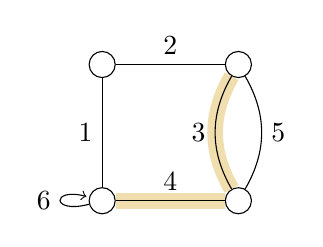
\begin{tikzpicture}
          \node[draw,circle] (r) at (0,0) {};
          \node[draw,circle] (q) at (0,1.73) {};
          \node[draw,circle] (w) at (1.73,1.73) {};
          \node[draw,circle] (t) at (1.73,0) {};
  
          \draw (q) -- node[above] {2} (w);
          \draw (q) -- node[left] {1} (r);
          \draw[preaction={draw=darktan, line width=2mm}] 
                (r) -- node[above] {4} (t);
          \path (t) 
          edge [bend left, preaction={draw=darktan, line width=2mm}] 
          node[left] {3} (w);
          \path (t) 
          edge [bend right]
          node[right] {5} (w);
          \path (r) 
          edge [loop left] 
          node[left] {6} (r);
      \end{tikzpicture}
      \caption{Agent $a_2$}
    \end{subfigure}
    \hfill
    \begin{subfigure}{0.3\textwidth}
      \centering
      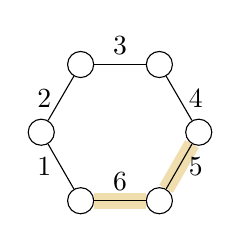
\begin{tikzpicture}        
          \node[draw, circle] (q) at (0,0)       {};
          \node[draw, circle] (w) at (1,0)       {};
          \node[draw, circle] (e) at (1.5,0.87)  {};
          \node[draw, circle] (r) at (1,1.73)    {};
          \node[draw, circle] (t) at (0,1.73)    {};
          \node[draw, circle] (y) at (-0.5,0.87) {};
  
          % Draw the edges
          \draw[preaction={draw=darktan, line width=2mm}] 
                (q) -- node[above] {6} (w);
          \draw[preaction={draw=darktan, line width=2mm}] 
                (w) -- node[right] {5} (e);
          \draw (e) -- node[right] {4} (r);
          \draw (r) -- node[above] {3} (t);
          \draw (t) -- node[left]  {2} (y);
          \draw (y) -- node[left]  {1} (q);
      \end{tikzpicture}
      \caption{Agent $a_3$}
    \end{subfigure}

    \caption{The resulting MMS-fair allocation after augmenting along $(2,4)$.}
    \label{fig:yes_mms}
  \end{figure}

Finally, after all agents have received their MMS, any remaining unallocated goods are simply allocated to agent 1. This ensures that the allocation is complete, though not necessarily clean. These goods, denoted $junk$ in Algorithm~\ref{alg:mms}, are the goods for which no agent has any additional value, either because they were always 0-valued or because every agent has achieved a basis in their matroid.

\pr{AlgMMS} highlights how strong fairness guarantees can be made when working with matroid-rank valuations. In the general, additive case, even computing the MMS of a single agent is NP-hard. With this algorithm, we can produce MMS-fair allocations in polynomial time.


\paragraph{Yankee Swap.}

\section{Matroid partitioning}
\label{sec:matroid-union-impl}
\subsection{Exchange graph}
\subsection{Shortest path}
\subsection{Transfer path augmentation}
\chapter{Using the library}
\label{chap:yankee-swap}
At this point in the report, I have described how Matroids.jl implements the functionality required for the empirical study of matroidal fair allocation algorithms. The previous chapters detailed three such algorithms---\pr{Envy-Induced-Transfers}, \pr{AlgMMS} and \pr{Yankee-Swap}---and described how Matroids.jl exposes the functions needed to implement these. Subsequently, I showed how Matroids.jl represents and randomly generates matroids. With random matroids and the functional requirements listed in Table~\ref{tab:algo_reqs} in hand, it is time to put the library to the test, and investigate whether it in fact des enable the implementation and empirical study of matroidal fair allocation algorithms.

This chapter serves a proof of concept for Matroids.jl, demonstrating the library's ability to facilitate the implementation and evaluation of matroidal fair allocation algorithms. As such, I will, in addition to describing the implementation of the algorithms, provide some experimental results regarding the fairness of the allocations produced. These algorithms are well-understood, so while the experimental results in this chapter may not represent novel findings, they serve as verification of the library's intended functionality, from random matroid generation, through fair allocation, to fairness evaluation. They should be considered proof that Matroids.jl is a tool that enables a new workflow for working programmatically with matroids in fair allocation, successfully extending Allocations.jl with capabilities to run previously inaccessible algorithms. The successful development of this tool is the main contribution of this thesis.

\section{Implementing Envy-induced transfers}
The pseudocode and high-level description of \pr{Envy-Induced Transfers} can be found in Section~\ref{sec:three-algos}. In this section, I will give a step-by-step explanation of my implementation of the algorithm.

The function accepts an instance of a fair allocation problem with matroid-rank valuations, represented with the \jlinl{MatroidRank} struct defined in Section~\ref{sec:fairness-impl}. Initially, a clean, MAX-USW allocation $A$ is found using the matroid partitioning algorithm whose implementation, \jlinl{matroid_partition_knuth73}, is described in Section~\ref{sec:matroid-union-impl}. This function returns a tuple $(A, junk)$, where $junk$ is the set of goods that did not fit into any independent bundle and is disregarded (\pr{Envy-Induced-Transfers} preferring cleanness over completeness). The partition is converted into an instance of \jlinl{Allocation}, which is provided by Allocations.jl. \pr{Envy-Induced-Transfers} continues until no agent envies another for more than one good; the envy between each pair of agents $i,j$ is represented with an $i\times j$-matrix \jlinl{envy} such that \jlinl{envy}$[i,j] = v_i(A_j) - v_i(A_i)$ holds agent $i$'s envy towards agent $j$. During each iteration a pair of agents $i,j$ is found such that \jlinl{envy}$[i,j] > 1$. Then, a good $g\in A_j$ with $\Delta_i(A_i, g)$ is transferred from $A_j$ to $A_i$. This is the envy-induced transfer from which the algorithm derives its name. After the transfer, the envy table is updated to reflect the new allocation.

The full implementation of \pr{Envy-Induced-Transfers} is given in Figure~\ref{code:Envy-Induced-Transfers}. This implementation highlights an important optimization when working programmatically with matroids, which is to not use the rank function on a set that is known to be independent. As seen in the implementations given in Chapter~\ref{chap:generating_matroids}, the rank function is expensive; \jlinl{rank(m::GraphicMatroid, S)}, for instance, runs Kruskal's algorithm as a subroutine, giving a time complexity of $O(|S|\lg{|S|})$ for finding the rank of $S$. When $S$ is independent, the rank is $|S|$---the size of a set can be found in constant time using \jlinl{length(S)}\footnote{From the Julia source code (base/set.jl): \jlinl{length(s::Set) = length(s.dict)}~\cite{bezanson2017julia}. A set, though itself unindexable, is represented behind the scenes in Julia as a dictionary, which is indexable and hence has a lastindex field, thus allowing the constant time length computation.}.

\begin{figure}[ht!]
\begin{jllisting}
function alloc_eit_bciz21(V::MatroidRank; partition=nothing)
  n = na(V); m = ni(V)

  if partition === nothing
    # Compute a clean, MAX-USW allocation.
    (partition, _junk) = matroid_partition_knuth73(V.Ms)
  end
  
  A = Allocation(n, m)
  for (i, bundle) in enumerate(partition)
    give!(A, i, bundle)
  end

  # Envy table envy[i,j] holds i's envy towards j, v_i(A_j) - v_i(A_i).
  envy = zeros(Int, n, n)
  for i in 1:n, j in 1:n
    # We use length when we know the bundles are independent.
    envy[i,j] = value(V, i, bundle(A, j)) - length(bundle(A, i))
  end

  # While there are agents i, j st i envies j more than 1...
  i,j = argmax(envy) |> Tuple
  while envy[i,j] > 1
    # Find item in A_j with marginal gain for i.
    for g in bundle(A,j)
      if Δ(V, A, i, g) == 1
        # Envy-induced transfer:
        deny!(A, j, g)
        give!(A, i, g)
    
        # Update D.
        for k in 1:n
          envy[i, k] = value(V, i, bundle(A, k)) - length(bundle(A, i))
          envy[k, i] = value(V, k, bundle(A, i)) - length(bundle(A, k))
          envy[j, k] = value(V, j, bundle(A, k)) - length(bundle(A, j))
          envy[k, j] = value(V, k, bundle(A, j)) - length(bundle(A, k))
        end

        break
      end
    end

    i,j = argmax(envy) |> Tuple
  end

  return A
end
\end{jllisting}
\caption{The Matroids.jl implementation of \pr{Envy-Induced-Transfers}}
\label{code:Envy-Induced-Transfers}
\end{figure}

The concept of a \textit{loop invariant} is useful for reasoning about the correctness of an algorithm, and can in this case be used to rigorously show that each bundle $A_i$ is independent in $\mathfrak{M}_i$ throughout the procedure. A loop invariant is a property that is true before the loop starts (initialization), remains true at the start of each iteration (maintenance) and is true upon termination~\cite{Cormen2009-zm}. \pr{Envy-Induced-Transfers} has a loop invariant stating that the allocation $A$ is clean, or, equivalently, that each $A_i$ is independent in $\mathfrak{M}_i$. This is true on initialization: \pr{Matroid-Partition} produces a clean, MAX-USW allocation. Each iteration, the algorithm a good $g$ such that $\Delta_i(A_i, g)$ is transferred from $A_j$ to $A_i$ for some agents $i,j$. Since $A_j$ is independent, $A_j-g$ is independent due to the hereditary property. Similarly, due to the exchange property, $A_i+g$ is also independent, and the loop invariant is maintained. The algorithm terminates when it has reached EF1, and $A$ is returned as-is, a clean allocation. This proves that it is a valid optimization to use \jlinl{length} instead of \jlinl{rank} when finding $v_i(A_i)$ in the implementation of this algorithm. Notice that \jlinl{value} (which in turn uses \jlinl{rank}---refer to Section~\ref{sec:fairness-impl} for details) is still used when checking $v_i(A_j)$ for $i\neq j$. 



A bundle will not necessarily be independent in another agent's matroid, hence \jlinl{rank} calls are still required when checking $v_i(A_j)$. To understand the effect of replacing half the \jlinl{rank} calls (the ones on sets known to be independent) with calls to \jlinl{length}, I ran the following simple experiment:
\begin{enumerate}
  \item Generate six random graphic matroids with 256 goods: \\\jlinl{m1 = GraphicMatroid(erdos_renyi(rand(128:512), 256))}
  \item Precompute the initial partition: \\\jlinl{(p, _) = matroid_partition_knuth73([m1,m2,m3,m4,m5,m6])}
  \item Run \jlinl{@btime alloc_eit_bciz21(V; partition=p)} with calls to \jlinl{length} where applicable
  \item Run \jlinl{@btime alloc_eit_bciz21(V; partition=p)} with only calls to \jlinl{value}
\end{enumerate}
On average, the version that always called \jlinl{value} took 181.5ms to compute, whereas the optimized version needed only 97.625ms. It is clear that the calls to \jlinl{value} takes up a significant portion of the runtime of the function, and replacing half of them with a constant-time call to \jlinl{length} is therefore a substantial improvement, shaving off roughly half the runtime.


\section{Implementing AlgMMS}
The next algorithm I implement in order to demonstrate the capabilities of Matroids.jl is \pr{AlgMMS}. Refer to Section~\ref{sec:three-algos} for the pseudocode and high-level description of the algorithm. The full source code of my implementation is given in Figure~\ref{code:AlgMMS}.

\begin{figure}[ht!]
\begin{jllisting}
function alloc_algmms_bv21(V::MatroidRank)
  n = na(V); m = ni(V)

  # Compute a clean, (partial) MAX-USW allocation.
  (partition, junk) = matroid_partition_knuth73(V.Ms)
  A = Allocation(n, m)
  for (i, bundle) in enumerate(partition)
    give!(A, i, bundle)
  end

  # Compute MMS of each agent.
  mmss = [mms_i(V, i) for i in 1:n]

  S_less = Set([i for i in 1:n if value(V, i, A) < mmss[i]])
  S_more = Set([i for i in 1:n if value(V, i, A) > mmss[i]])

  D = exchange_graph(V.Ms, A)

  while length(S_less) > 0
    # i is an agent with less than their maximin share.
    i = popfirst!(collect(S_less))

    # The goods for which i has positive marginal value.
    F_i = [g for g in 1:m if is_indep(V.Ms[i], bundle(A, i) ∪ g)]
    A_more = reduce(∪, [bundle(A, j) for j in S_more])

    transfer_path = find_shortest_path(D, F_i, A_more)
    @assert transfer_path !== nothing

    j = owner(A, transfer_path[end]) # The losing agent.
    
    transfer!(V.Ms, D, A, i, transfer_path)

    # Only i and j have received a new value.
    for k in [i,j]
      if value(V,k,A) < mmss[k] push!(S_less, k) else setdiff!(S_less, k) end
      if value(V,k,A) > mmss[k] push!(S_more, k) else setdiff!(S_more, k) end
    end
  end

  # Give agent 1 any unallocated items (these are 0-valued by everyone).
  give!(A, 1, junk)
  return A
end
\end{jllisting}
\caption{The Matroids.jl implementation of \pr{AlgMMS}}
\label{code:AlgMMS}
\end{figure}

The function accepts an instance of a fair allocation problem with matroid-rank valuations, and outputs a clean, MAX-USW, MMS-fair allocation. If not passed in the optional parameter \jlinl{partition}, an initial clean and MAX-USW allocation $A$ is computed with \jlinl{matroid_partition_knuth73}, identically to how \jlinl{alloc_eit_bciz21} starts off. The maximin share $\mu_i$ is computed for each agent $i$, using the function \jlinl{mms_i}, whose implementation is given in Figure~\ref{code:mms_i}. Next, the setup phase, the algorithm finds \jlinl{S_less}, the set of agents whose bundle value in $A$ is less than their maximin share, and \jlinl{S_more}, the set of agents whose bundle value is higher. Finishing off the setup phase, the exchange graph of the allocation is produced with the function \jlinl{exchange_graph} from Figure~\ref{code:exchange_graph}.

Each iteration, an agent $i$ such that $A_i<\mu_i$ is popped from \jlinl{S_less}. The set of goods $g$ such that $\Delta_i(A_i, g) = 1$ is computed, this is the set \jlinl{F_i}. A shortest path is found from the goods in \jlinl{F_i} to the goods belonging to agents in \jlinl{S_more} using \jlinl{find_shortest_path}, which either returns a transfer path or \jlinl{nothing} if none could be found. In the paper describing AlgMMS, Barman and Verma show that such a path always exist as long as someone has less than their maximin share. A new allocation is acquired by calling \jlinl{transfer!}, passing it the list of matroids, the exchange graph, the allocation, the agent whose bundle value is about to improve and the transfer path. \jlinl{transfer!} updates the exchange graph and allocation in place (hence the exclamation mark---a Julia convention). \jlinl{S_less} and \jlinl{S_more} are updated for the agents whose bundle value has changed. When \jlinl{S_less} is empty, the while loop terminates, the first agent is granted the goods that were not allocated by \jlinl{matroid_partition_knuth73} and the resulting allocation is returned.

\jlinl{alloc_algmms_bv21} is another example showing that it is often unnecessary to compute the actual value (entailing an expensive call to \jlinl{rank}) of a bundle. Notice that, when finding the list of positively marginal-valued good $F_i$ for agent $i$, the $\Delta_i$ function is not chosen for the task. The algorithm has the same loop invariant as \pr{Envy-Induced-Transfers} regarding the cleanness of $A$ at every step of the algorithm; thus, $F_i$ is simply the list of goods such that $A_i + g$ is independent. 

\section{Implementing Yankee Swap}
\pr{Yankee-Swap} is the third and final algorithm whose implementation will serve as a proof of the capabilities of Matroids.jl. \pr{Yankee-Swap} differs from the previous two algorithms in that it does not start out with a clean, MAX-USW allocation procured with \pr{Matroid-Partition}, instead adding a new ``agent zero'', whose bundle is the pot of unallocated items. Agent zero is represented with a \jlinl{ZeroMatroid}, the special case of the uniform matroid in which only the empty set is independent. This ensures that the goods allocated to agent zero are sinks on the graph, with no out-edges.

The source code for my implementation of \pr{Yankee-Swap} is given in Figure~\ref{code:Yankee-Swap}. The function proceeds similarly to \pr{AlgMMS}. Each iteration, a least-fortunate, highest-priority agent $i$ is chosen from among the agents whose bundle value can still improve (denoted with the \jlinl{flag} array). The set $F_i$ of goods for which $i$ has positive marginal value is found, and a transfer path is produced between $F_i$ and the set of goods currently belonging to agent zero (the unallocated goods). The next allocation is produced by augmenting along the transfer path and the next iteration starts if some agent can still improve their bundle; otherwise it terminates.

\begin{figure}[ht!]
\begin{jllisting}
function alloc_yankee_swap_vz22(V::MatroidRank)
  n = na(V); m = ni(V)

  # Randomly prioritize the agents.
  agents = shuffle(1:n)

  # Agent "0" (n+1) has a corresponding zero matroid.
  Ms_ = [V.Ms..., ZeroMatroid(m)]

  A = Allocation(n+1, m)
  give!(A, n+1, 1:m) # The bundle of unallocated items.
  flag = falses(n)

  D = exchange_graph(Ms_, A)

  while false in flag
    # The agents whose bundle can still improve.
    T = [i for i in agents if flag[i] == false]
    
    # Find the agents in T with minimim value.
    T_vals = [(i, length(bundle(A, i))) for i in T]
    min_val = minimum(last, T_vals)
    T_ = [i for (i, v) in T_vals if v == min_val]

    # The highest priority agent with minimum value.
    i = T_[1] 

    # The goods for which i has positive marginal value.
    F_i = [g for g in 1:m if is_indep(V.Ms[i], bundle(A, i) ∪ g)]

    #  a shortest path from F_i to an unallocated good.
    A_0 = [g for g in 1:m if owner(A, g) == n+1]
    transfer_path = find_shortest_path(D, F_i, A_0)

    # Transfer if path exists.
    if transfer_path !== nothing
      transfer!(Ms_, D, A, i, transfer_path)
    else
      flag[i] = true
    end
  end
  
  return A
end
\end{jllisting}
\caption{The Matroids.jl implementation of \pr{Yankee-Swap}}
\label{code:Yankee-Swap}
\end{figure}

\section{Running some experiments}
\label{chap:results}
At this point, it seems like Matroids.jl has achieved its goal of making it easy to implement matroidal fair allocation algorithms. The arcane matroid logic is safely hidden away behind semantically named functions in the library's, allowing the developer to focus on the business logic of the algorithm at hand. Of course, the real purpose of Matroids.jl is to enable the empirical study of matroidal fair allocation algorithms. Let us now turn our attention to how an experimental setup might be implemented. In this section, we will use the functionality available to us in the current, proof-of-concept version of Matroids.jl to investigate how the three algorithms we have implemented perform on a range of fairness criteria. These results, though probably not terribly interesting in and of themselves, should serve to illustrate that Matroids.jl does in fact live up to its purpose in life; namely, to be a practical, empirical tool to be used alongside the abundant kit of theoretical tools afforded by matroid theory.

The experimental plan is as follows:
\begin{enumerate}
  \item Generate a matroid-rank-valued fair allocation instance with $n$ matroids over $m$ elements.
  \item Find an allocation using some allocation algorithm.
  \item Check the resulting allocations against some set of approximate fairness notions.
  \item Repeat steps 1-3 $k$ times and present the average results.
\end{enumerate}

\begin{figure}
  \begin{jllisting}
function gen_matroidrank_profile(n, gen_matroid, T)
  function gen()
    ms = Array{T}(undef, n)

    Threads.@threads for i in 1:n
      ms[i] = gen_matroid()
    end

    return MatroidRank(ms, m)
  end

  return gen
end
  \end{jllisting}
  \caption{Function to initialize a random matroid-rank valuation profile, given a random matroid generator}
  \label{code:gen_matroidrank_profile}
\end{figure}

Figure~\ref{code:gen_matroidrank_profile} shows a Julia function that accepts a function that generates a matroid, and returns a function that constructs a matroid-rank valuation profile with $n$ thusly generated matroids. Matroid generation is rather slow, so the matroids are generated in parallel\footnote{Depending on how many threads are available. Julia starts single-threaded by default, but supports multi-threading~\cite{bezanson2017julia}.}. By plugging in a function for generating random graphs with $m$ edges, as given in Figures~\ref{code:random_ba_graph}, \ref{code:random_ws_graph} and \ref{code:random_er_graph}, we can generate a valuation profile consisting of graphic matroids. Alternatively, we can pass in \jlinl{random_knuth_matroid} to generate a profile of matroids given via their closed sets representations. 
\chapter{Generating matroids}
\label{chap:generating_matroids}
The overarching goal for this project is to make Matroids.jl, a proof-of-concept library for working programmatically with matroids, specifically in the context of fair allocation. This chapter covers how Matroids.jl enables the creation of specific matroids and the generation of random ones, as well as how to access important properties such as independent sets, closed sets, circuits, bases, the rank function and the closure function. The first part of the chapter focuses on implementing these features for various types of matroids, including uniform, linear (vector), graphic, and partition matroids. The final part of the chapter is a significant portion of the thesis as a whole, and describes the implementation of Knuth's interesting algorithm~\cite{knuth-1975} for the erection of arbitrary rank-$r$ matroids.

\begin{enumerate}
  \item \jlinl{rank}
  \item \jlinl{closure}
  \item \jlinl{bases}
  \item \jlinl{is_indep}
  \item \jlinl{is_circuit}
  \item \jlinl{is_basis}
\end{enumerate}


\section{Uniform matroids and partition matroids}
A uniform matroid $U_n^r$ is the matroid over $n$ elements where the independent sets are exactly the sets of cardinality at most $r$. The free matroid $U_n^n = (E, 2^E)$ is a special case of the uniform matroid and is the simplest, biggest and least interesting type of matroid, being the trivial case in which every subset of $E$ is an independent set. In Matroids.jl, we represent uniform matroids with a simple struct.

\begin{jllisting}
struct UniformMatroid
  n::Integer
  r::Integer
end

FreeMatroid(n) = UniformMatroid(n, n)
\end{jllisting}


\section{Linear matroids}

\section{Graphic matroids}
We begin with defining the graph theory terms used in this section. An undirected graph $G=(V,E)$ is said to be \textit{connected} if there exists at least one path between each pair of nodes in the graph; otherwise it is \textit{disconnected}. A disconnected graph consists of at least two connected subsets of nodes. These connected subgraphs are called \textit{components}. A \textit{tree} is a connected acyclic graph, and a \textit{forest} is a disconnected graph consisting of some number of trees. A \textit{spanning tree} of $G$ is a subgraph with a unique simple path between all pairs of vertices of $G$. A \textit{spanning forest} of $G$ is a collection of spanning trees, one for each component. The \textit{degree} of a node $v$ is the number of edges for which $v$ is an endpoint. A \textit{regular graph} is a graph in which all nodes have the same degree. An \textit{induced subgraph} $G[S]$, where $S$ is either a subset of the nodes of $G$ (in which case $G[S]$ is a \textit{node-induced subgraph}) or of the edges of $G$ (\textit{edge-induced}).

Given a graph $G=(V,E)$, let $\mathcal{I} \subseteq 2^E$ be the family of subsets of the edges $E$ such that, for each $I \in \mathcal{I},\ (V, I)$ is a forest. It is a classic result of matroid theory that $\mathfrak{M} = (E, \mathcal{I})$ is a matroid~\cite[p.~657]{schrijver-2003}. To understand how, we will show that it adhers to axioms (1) and (2'), as given in Section~\ref{sec:matroid-theory}. (1) holds trivially, as all subsets of a forest are forests. To see that (2') holds, consider the bases $\mathcal{B} \subseteq \mathcal{I}$. By definition, each basis $B \in \mathcal{B}$ is a maximal forest over $G$. Since a spanning tree of a graph with $n$ nodes must needs have $n-1$ edges, we have $|B| = |V| - k$, where $k$ is the number of components of $G$. This is the same for every $B \in \mathcal{B}$, which proves property (2'). Any matroid given by a graph $G$, denoted by $\mathfrak{M}(G)$, is called a \textit{graphic matroid}.

\subsection{Random graphs}
Since generating random graphic matroids will require us to generate random graphs, let us take a look at some of the options available to us for this. Luckily for us, random graphs has been an area of extensive study for more than sixty years, and several models with different properties exist.

The Erdős-Rényi (ER) model (also known as Erdős-Rényi-Gilbert~\cite{fienberg-2012}) picks uniformly at random a graph from among the $\binom{\binom{n}{2}}{M}$ possible graphs with $n$ nodes and $M$ edges, or, alternatively, constructs a graph with $n$ nodes where each edge is present with some probability $p$~\cite{erdos-1959, gilbert-1959}. This model produces mostly disconnected graphs, and the size distribution of its components with respect to the number of edges has been studied extensively. With $n$ nodes and fewer than $\frac{n}{2}$ edges, the resulting graph will almost always consist of components that are small trees or contain at most one cycle. As the number of edges exceeds $\frac{n}{2}$, however, the so-called ``giant'' component of size $\mathcal{O}(n)$ emerges, and starts to absorb the smaller components~\cite{janson1993birth}. The ER model is the oldest and most basic random graph model, and is often referred to simply as the random graph, denoted by $G(n,p)$.

Variations of the ER model have been developed by physicists and network scientists to produce phenomena commonly seen in real-world networks~\cite{fienberg-2012}. These variations include the Barabási-Albert model, which grows an initial connected graph using preferential attachment (a mechanism colloquially known as ``the rich get richer''), in which more connected nodes are more likely to receive new connections. This results in graphs in which a small number of nodes (``hubs'') have a significantly higher degree than the rest, creating a power-law distribution of node degrees. This property is known as scale-freeness and is thought to be a characteristic of the Internet~\cite{barabasi-albert}. 

Another approach is the Watts-Strogatz model, which starts with a ring lattice, a regular graph with $n$ nodes, each with degree $k$, and then rewires each edge with some probability $p$. By changing $p$, one is able to `tune' the graph between regularity (p=0) and disorder (p=1). For intermediate values of $p$, Watts-Strogatz produces so-called ``small-world'' graphs, which exhibit both a high degree of clustering (how likely two nodes with a common neighbor are to be adjacent), and short average distance between nodes. This phenomenon is found in many real-world networks, such as social systems or power grids~\cite{Watts-1998}.

\subsection{Properties of random graphic matroids}
We will use the Graphs.jl library~\cite{Graphs2021} for handling graphs in Matroids.jl. This library has built-in methods for the random graph models described in the previous chapter\footnote{\href{https://docs.juliahub.com/Graphs/VJ6vx/1.4.1/generators/}{https://docs.juliahub.com/Graphs/VJ6vx/1.4.1/generators/}}. 

When constructing matroids, we want to be able to specify the size of the ground set, and perhaps also the rank of the matroid. Let us see how we can achieve this with the random graph models we have discussed. The method \jlinl{barabasi_albert(n,k)} generates a Barabási-Albert model random graph with $n$ nodes. It starts with an initial graph of $k$ nodes, and adds the remaining $n-k$ nodes one at a time, each new node receiving $k$ edges via preferential attachment. Thus, the final graph has $|E| = (n-k)k$ edges. To specify a matroid with $m$ edges, we pick some $k|m$ and solve for $n$. Remember that the rank of a graphic matroid is the size of a spanning tree over the graph, which is $n-1$ when the graph is connected. If we select a smaller $k$ from among the factors of $|E|$, we get a larger final rank, and vice versa. We can generate a Watts-Strogatz model random graph with the method \jlinl{watts_strogatz(n, k, β)}, where $n$ is the number of nodes, $k$ the node degree and $\beta$ the probability of rewiring. The number of edges of a regular graph with $n$ nodes and degree $k$ (and thus the size of the ground set of the induced graphic matroid) is given by $\frac{nk}{2}$, so $nk$ must be even. Erdős-Rényi is the simplest model for our purposes, as the method \jlinl{erdos_renyi(nv, ne)} simply takes in the desired number of nodes and edges. However, since the resulting graph has a large number of components for $|E| < \frac{n}{2}$, we have less fine-grained control over the final rank of the induced graphic matroid.

In Matroids.jl, we ``generate'' a graphic matroid by simply accepting some graph, and figure out the rank of the matroid using Kruskal's algorithm for maximal spanning forests, which runs in $\mathcal{O}(|E| \lg |E|)$ time~\cite{Cormen2009-zm}. Implementing the methods for finding the properties of our graphic matroids is simple, as they reduce to well-known algorithms (implemented by Graphs.jl) for finding the properties of the graphs they are derived from. 

\begin{jllisting}
using Graphs

struct GraphicMatroid
  g::Graph
  n::Integer
  r::Integer
  GraphicMatroid(g::Graph) = new(g, ne(g), length(kruskal_mst(g)))
end
\end{jllisting}

\textbf{The rank function} returns the size of a spanning forest of the subgraph induced by some subset of the edges. This is the rank of that subset. Thus, the rank of a subset $S \subseteq E$ can be found in $\mathcal{O}(|S| \lg |S|)$ time (when the MST is found using Kruskal's algorithm).

\begin{jllisting}
function rank(m::GraphicMatroid, S)
  edgelist = [e for (i, e) in enumerate(edges(g)) if i in S]
  subgraph, _vmap = induced_subgraph(m.g, edgelist)
  return length(kruskal_mst(subgraph))
end
\end{jllisting}

\textbf{The indepence oracle} returns whether the subgraph induced by a supplied subset of edges is acyclic. While independence can also be determined with the rank function, by checking whether the cardinality of a set equals its rank, this uses a DFS behind the scenes\footnote{\href{https://docs.juliahub.com/Graphs/VJ6vx/1.4.1/pathing/\#Graphs.is\_cyclic}{https://docs.juliahub.com/Graphs/VJ6vx/1.4.1/pathing/\#Graphs.is\_cyclic}}, which runs in linear time~\cite{Cormen2009-zm}.

\begin{jllisting}
function is_indep(m::GraphicMatroid, S)
  edgelist = [e for (i, e) in enumerate(edges(g)) if i in S]
  subgraph, _vmap = induced_subgraph(m.g, edgelist)
  return !is_cyclic(subgraph)
end
\end{jllisting}

\textbf{The circuit oracle} \skelline
\begin{jllisting}
function is_circuit(m::GraphicMatroid, S)
  #TODO
end
\end{jllisting}

\textbf{The closure function} accepts a set of elements $S$, and returns the largest set of elements $\fn{cl}(S)$ such that $S \subseteq \fn{cl}(S) \subseteq E, \fn{r}(S) = r(cl(S))$. In a graph context, given a graph $G=(V,E)$ and an edge-induced subgraph $G[S] = (V´, S), S\subseteq E$, this is the same as finding the largest edge-induced subgraph $G[T], S\subseteq T\subseteq E$, in which a spanning tree has the same number of edges as one in $G[S]$. Since the size of a spanning tree in $G[S]$ is given by $|V´|-1$, $G[T]$ cannot contain any edges to nodes not in $V´$, as this would increase the rank of $G[T]$. Therefore, we get that the closure of $S$ is the largest set $T$ of edges between nodes that are present in the edge-induced subgraph $G[S]$. The method \jlinl{closure} below returns the set of all edges whose endpoints are both located in the subgraph induced by $S$.
\begin{jllisting}
function closure(m::GraphicMatroid, S)
  edgelist = [e for (i, e) in enumerate(edges(m.g)) if i in S]
  _sg, vmap = induced_subgraph(m.g, edgelist)
  return [e for e in edges(m.g) if [e.src, e.dst] ⊆ vmap]
end
\end{jllisting}

\section{Knuth's matroid construction}
\label{sec:kmc}
In the preparatory project to this thesis, delivered to my advisor in the fall of 2022, I implemented Knuth's 1974 algorithm for the random generation of arbitrary matroids via the erection of closed sets \cite{knuth-1975}. With this, I was able to randomly generate matroids of universe sizes $n \leq 12$, but for larger values of $n$ my implementation was unbearably slow. In this section, Knuth's method for random matroid construction will be described, along with the steps I have taken to speed up my initial, naïve implementation.

\pr{Knuth-Matroid} (given in Algorithm~\ref{alg:knuth}) accepts the ground set $E$ and a list $\mathrm{X}$ such that $\mathrm{X}[i] \subseteq 2^E$, and produces the rank-$r$ matroid $\mathfrak{M}$ such that $\mbox{rank}(X) = k$ for each $X \in \mathrm{X}[k]$. This is done in a bottom-up manner through $r$ sequential erections starting from the empty rank-0 matroid, $\mathfrak{M}^{(0)}$, each iteration $i$ producing the erection $\mathfrak{M}^{(i+1)}$ from $\mathfrak{M}^{(i)}$ and $\mathrm{X}[i]$. The algorithm outputs the tuple $(E, \mathrm{F})$, where $\mathrm{F} = [F_0, \ldots, F_r]$, $r$ being the final rank of $\mathfrak{M}$ and $F_i$ the family of closed sets of rank $i$. In the paper, Knuth shows that $\bigcup_{i=0}^r \mathrm{F}[r] = \mathcal{F}$, where $\mathcal{F}$ is the set of closed sets of a matroid, and so the algorithm produces a valid matroid represented by its closed sets.

\begin{algorithm}[float*=ht!]{\pr{Knuth-Matroid}(E, \mathrm{X})}{knuth}

  \textbf{Input:}     \tab The ground set of elements $E$, and a list of enlargements $\mathrm{X}$.

  \textbf{Output:}    \tab The list of closed sets of the resulting matroid grouped by rank, \\
  \mbox{}\tab $\mathrm{F} = [F_0, \ldots, F_r]$, where $F_i$ is the set of closed sets of rank $i$.

  \begin{pseudo}[kw, label=\small\arabic*, indent-mark, line-height=1.2]
    $r = 0, \mathrm{F} = [\{ \emptyset \}]$ \\
    while \cn{true}  \\+
    $\pr{Push!}(\mathrm{F}, \pr{Generate-Covers}(\mathrm{F}, r, E))$ \\
    $\mathrm{F}[r+1] = \mathrm{F}[r+1] \cup \mathrm{X}[r+1]$ \\
    \pr{Superpose!}(\mathrm{F}[r+1], \mathrm{F}[r]) \\

    if $E \not \in F[r+1]$ \\+
    $r \leftarrow r+1$ \\-
    else \\+
    return $(E, \mathrm{F})$

  \end{pseudo}

\end{algorithm}

To understand the procedure, let us investigate what Algorithm~\ref{alg:knuth} does at iteration $1<i<r$, where $r$ is the final rank $\mathfrak{M}$, the matroid under construction. At iteration $i$, we produce a rank-$(i+1)$ erection $\mathfrak{M}^{(i+1)}$ of $\mathfrak{M}^{(i)}$, which is represented by its closed sets $\mathrm{F} = [F_0, F_1, ..., F_i]$, where $F_i$ is the set of closed sets of rank $i$. We want to produce the set $F_{i+1}$ of rank-$r$ closed sets of an erection of $\mathfrak{M}^{(i)}$ such that each $X \in \mathrm{X}[i]$ is contained in some rank-$r$ closed set. First we find the ``covers'' of each closed set in $F_i$. The covers of a closed set $A$ of rank $r$ are the sets obtained by adding one more element from $E$ to $A$. The covers are generated with \pr{Generate-Covers}(\mathrm{F}, r, E).

\begin{tcolorbox}[pseudo/boxruled]
  \begin{pseudo}*
    \hd{Generate-Covers}(\mathrm{F}, r, E) \\
    return $\{ A \cup \{a\} : A \in \mathrm{F}[r], a \in E \setminus A \}$
  \end{pseudo}
\end{tcolorbox}

Given no enlargements ($\mathrm{X}[i] = \emptyset$), the resulting matroid $\mathfrak{M}^{(i+1)}$ is the \textit{free erection} of $\mathfrak{M}^{(i)}$, and there are no essential closed sets in $F_{i+1}$. Arbitrary matroids can be generated by supplying different lists $\mathrm{X}$. When enlarging, the sets in $\mathrm{X}[r+1]$ are simply added to $\mathrm{F}[r+1]$, before \pr{Superpose!} is run to ensure that the newly enlarged family of closed sets of rank $r+1$ is valid (ie. in accordance with the closed set axioms given in Section~\ref{sec:matroid-theory}). If $F_{r+1}$ contains two sets $A,B$ whose intersection $A \cap B \not \subseteq C$ for any $C \in F_{r}$ (in other words, their intersection is not a closed set), replace $A,B$ with $A \cup B$. Repeat until no two sets exist in $F_{r+1}$ whose intersection is not contained within some set $C \in F_{r}$.

\begin{tcolorbox}[pseudo/filled, colback=lighttan, float*=ht!]
  \begin{pseudo}[kw, indent-mark, compact]*
    \hd{Superpose!}({F_{r+1},F_r}) \\
    for $A \in F_{r+1}$ \\+
    for $B \in F_{r+1}$ \\+
    \id{flag} $\leftarrow$ \cn{true} \\
    for $C \in F_r$ \\+
    if $A \cap B \subseteq C$ \\+
    \id{flag} $\leftarrow$ \cn{false} \\--
    \\
    if \id{flag} = \cn{true} \\+
    $F_{r+1} \leftarrow F_{r+1} \setminus \{A, B \}$ \\
    $F_{r+1} \leftarrow F_{r+1} \cup \{A \cup B \}$
  \end{pseudo}
\end{tcolorbox}


\subsection{Randomized KMC}
In the randomized version of \pr{Knuth-Matroid}, we generate matroids by applying a supplied number of random coarsening steps, instead of enlarging with supplied sets. This is done by applying \pr{Superpose!} immediately after adding the covers, then choosing a random member $A$ of $\mathrm{F}[r+1]$ and a random element $a \in E \setminus A$, replacing $A$ with $A \cup \{a\}$ and finally reapplying \pr{Superpose!}. The parameter $p = (p_1, p_2, \ldots)$ gives the number of such coarsening steps to be applied at each iteration of the algorithm.

The pseudocode descriptions of Knuth's matroid construction hews closely to the initial Julia implementation. It should already be clear that this brute force approach leads to poor performance---for instance, the \pr{Superpose!} method uses a triply nested for loop, which seems like a candidate for significant improvement. Section~\ref{sec:improving-performance} describes the engineering work done to create a more performant implementation.

\begin{algorithm}[float*=ht!]{\pr{Randomized-Knuth-Matroid}(E, p)}{rkmc}

  \textbf{Input:}     \tab The ground set of elements $E$, and a list $p = [p_1, p_2, ...]$, where \\
  \mbox{}\tab $p_r$ is the number of coarsening steps to apply at rank $r$ in the \\
  \mbox{}\tab construction.

  \textbf{Output:}    \tab The list of closed sets of the resulting matroid grouped by rank, \\
  \mbox{}\tab $\mathrm{F} = [F_0, \ldots, F_r]$, where $F_i$ is the set of closed sets of rank $i$.

  \begin{pseudo}[label=\small\arabic*, indent-mark, line-height=1.2]
    $r = 0, \mathrm{F} = [\{ \emptyset \}]$ \\
    \kw{while} \cn{true}  \\+
      $\pr{Push!}(\mathrm{F}, \pr{Generate-Covers}(\mathrm{F}, r, E))$ \\
      \pr{Superpose!}(\mathrm{F}[r+1], \mathrm{F}[r]) \\
      
      \kw{if} $E \in \mathrm{F}[r+1]$ \kw{return} $(E, \mathrm{F})$ \\
      
      \kw{while} $p[r] > 0$ \\+
        $A \leftarrow$ a random set in $\mathrm{F}[r+1]$ \\
        $a \leftarrow$ a random element in $E \setminus A$ \\
        \kw{replace} $A$ with $A \cup \{a\}$ in $\mathrm{F}[r+1]$ \\
        \pr{Superpose!}(\mathrm{F}[r+1], \mathrm{F}[r]) \\

        \kw{if} $E \in \mathrm{F}[r+1]$ \kw{return} $(E, \mathrm{F})$ \\

        $p[r] = p[r] - 1$ \\-
      $r = r + 1$

  \end{pseudo}

\end{algorithm}


\subsection{Improving performance}
\label{sec:improving-performance}
In the preparatory project to this thesis, I was able to recreate Knuth's table of observed mean values for the randomly generated matroids, but I was dismayed to find that my implementation was unable to handle matroids whose ground sets were even just a few elements larger. Considering that Knuth was able to run his experiments on the hardware available to him in the 1970s, I concluded that my implementation had room for improvement. Table~\ref{tab:perf_v1} shows the performance of my first implementation.

\begin{table}[ht!]
  \centering
    \begin{tabular}{llllllllll}
      \toprule
      $n$ & $(p_1, p_2, \ldots)$ & Trials & Time  & GC Time & Bytes allocated \\
      \midrule
        10 & (0, 6, 0)    & 100 & 0.0689663   & 0.0106786 & 147.237 MiB \\
        10 & (0, 5, 1)    & 100 & 0.1197194   & 0.0170734 & 251.144 MiB \\
        10 & (0, 5, 2)    & 100 & 0.0931822   & 0.0144022 & 203.831 MiB \\
        10 & (0, 6, 1)    & 100 & 0.0597314   & 0.0094902 & 132.460 MiB \\
        10 & (0, 4, 2)    & 100 & 0.1924601   & 0.0284532 & 406.131 MiB \\
        10 & (0, 3, 3)    & 100 & 0.3196838   & 0.0463972 & 678.206 MiB \\
        10 & (0, 0, 6)    & 100 & 1.1420602   & 0.1671325 & 2.356 GiB   \\
        10 & (0, 1, 1, 1) & 100 & 2.9283978   & 0.3569357 & 5.250 GiB   \\
        13 & (0, 6, 0)    & 10  & 104.0171128 & 9.9214449 & 161.523 GiB \\
        13 & (0, 6, 2)    & 10  & 11.4881308  & 1.3777947 & 20.888 GiB  \\
        16 & (6, 0, 0)    & 1   & -           & -         & -           \\
      \bottomrule
    \end{tabular}
  \caption{Performance of $\texttt{random\_kmc\_v1}$.}
  \label{tab:perf_v1}
\end{table}

The performance was measured using Julia's \jlinl{@timed}\footnote{\href{https://docs.julialang.org/en/v1/base/base/\#Base.@timed}{https://docs.julialang.org/en/v1/base/base/\#Base.@timed}} macro, which returns the time it takes to execute a function call, how much of that time was spent in garbage collection and the number of bytes allocated. The experiments was run on a 2021 MacBook Pro with the Apple M1 chip and 16GB RAM. As is evident from the data, larger matroids are computationally quite demanding to compute with this current approach, and the time and space requirements scales exponentially with $n$.

\subsubsection{Representing sets as binary numbers}
The first improvement we will attempt is to represent our closed sets using one of Julia's \jlinl{Integer} types of bit width at least $n$, instead of as a \jlinl{Set}\footnote{\href{https://docs.julialang.org/en/v1/base/collections/\#Base.Set}{https://docs.julialang.org/en/v1/base/collections/\#Base.Set}} of elements of $E$. Appendix~\ref{apx:code} contains all the code referenced in this chapter; the Julia implementation at this point can be found in \ref{apx:randkmcv2}. 

The idea is to define a family of closed sets of the same rank as \jlinl{Set\{UInt16\}}. Using \jlinl{UInt16} we can support ground sets of size up to 16. Each 16-bit number represents a set in the family. For example, the set $\{ 2,5,7 \}$ is represented by $$164 = 0\rm{x}00\rm{a}4 = 0\rm{b}0000000010100100 = 2^7+2^5+2^2.$$ At either end we have $\emptyset \equiv 0\rm{x}0000$ and $E \equiv 0\rm{xffff}$ (if $n = 16$). The elementary set operations we will need have simple implementations using bitwise operations.

\begin{table}[!ht]
  % \caption{Set operations and their equivalent bitwise operations}
  \centering
  \begin{tabular}{|l|l|}
  \hline
      Set operation & Bitwise operation \\\hline
      $A \cap B$      & $A$ AND $B$ \\\hline
      $A \cup B$      & $A$ OR $B$ \\\hline
      $A \setminus B$ & $A$ AND NOT $B$ \\\hline
      $A \subseteq B$ & $A$ AND $B$ = $A$ \\\hline
  \end{tabular}
\end{table}

We can now describe the bitwise versions of the required methods. The bitwise implementation of \pr{Generate-Covers} finds all elements in $E \setminus A$ by finding each value $0\leq i< n$ for which \jlinl{A & 1 << i === 0}, meaning that the set represented by \jlinl{1 << i} is not a subset of A. The bitwise implementation of \pr{Superpose!} is unchanged apart from using the bitwise set operations described above.

\begin{table}[ht!]
  \centering
  \begin{tabular}{llllllllll}
    \toprule
    $n$ & $(p_1, p_2, \ldots)$ & Trials & Time  & GC Time & Bytes allocated \\
    \midrule
    10 & [0, 6, 0] & 100 & 0.0010723 & 0.0001252 & 1.998 MiB \\ 
    10 & [0, 5, 1] & 100 & 0.0017543 & 0.0001431 & 3.074 MiB \\ 
    10 & [0, 5, 2] & 100 & 0.0008836 & 0.0001075 & 2.072 MiB \\ 
    10 & [0, 6, 1] & 100 & 0.0007294 & 6.73e-5 & 1.700 MiB \\ 
    10 & [0, 4, 2] & 100 & 0.0020909 & 0.0001558 & 3.889 MiB \\ 
    10 & [0, 3, 3] & 100 & 0.0024636 & 0.0002139 & 4.530 MiB \\ 
    10 & [0, 0, 6] & 100 & 0.007082 & 0.0004801 & 9.314 MiB \\ 
    10 & [0, 1, 1, 1] & 100 & 0.0132477 & 0.0008307 & 17.806 MiB \\ 
    13 & [0, 6, 0] & 10 & 0.042543 & 0.0014988 & 31.964 MiB \\ 
    13 & [0, 6, 2] & 10 & 0.0183313 & 0.0012176 & 21.062 MiB \\ 
    16 & [0, 6, 0] & 10 & 1.2102877 & 0.0146129 & 450.052 MiB \\ 
    \bottomrule
  \end{tabular}
  \caption{Performance of $\texttt{random\_kmc\_v2}$.}
  \label{tab:perf_v2}
\end{table}

The performance of \mono{random\_kmc\_v2} is shown in Table~\ref{tab:perf_v2}. It is clear that representing closed sets using binary numbers represents a substantial improvement -- we are looking at performance increases of 100x-1000x across the board.


\subsubsection{Sorted superpose}
Can we improve the running time of our implementation further? It is clear that \pr{Superpose!} takes up a large portion of the compute time. In the worst case, when no enlargements have been made, $F_{r+1}$ is the set of all $r+1$-sized subsets of $E$, $|F_{r+1}| = {\binom{n}{r+1}}$. Comparing each $A,B \in F_{r+1}$ with each $C \in F_r$ in a triply nested for loop requires $\mathcal{O}({\binom{n}{r+1}}^2{\binom{n}{r}})$ operations. In the worst case, no enlargements are made at all, and we build the free matroid in $\mathcal{O}(2^{3n})$ time (considering only the superpose step).

After larger closed sets have been added to $\mathrm{F}[r+1]$, \pr{Superpose!} will cause sets to merge, so that only maximal dependent sets remain. Some sets will even simply disappear. In the case where $X=\{1,2\}$ was added by \pr{Generate-Covers}, and the $Y=\{1,2,3\}$ was added manually as an enlargement, the smaller set will be fully subsumed in the bigger set, as $\{1,2\}\cap\{1,2,3\}=\{1,2\}$ (which is not a subset of any set in $\mathrm{F}[r]$) and $\{1,2\}\cup\{1,2,3\}=\{1,2,3\}$. In this situation, $Y$ would ``eat'' the covers $\{1,3\}$ and $\{2,3\}$ as well. This fact is reflected in the performance data -- compare the memory allocation differences between the 10-element matroid with $p=[0,0,6]$ and the one with $p=[0,6,0]$ in any of the performance tables in this section. Making enlargements at earlier ranks result in smaller matroids as more sets get absorbed.

\begin{jllisting}
function sorted_bitwise_superpose!(F, F_prev)
  As = sort!(collect(F), by = s -> length(bits_to_set(s)))
  while length(As) !== 0
    A = popfirst!(As)

    for B in setdiff(F, A)
      if should_merge(A, B, F_prev)
        insert!(As, 1, A | B)
        setdiff!(F, [A, B])
        push!(F, A | B)
        break
      end
    end
  end

  return F
end
\end{jllisting}

Since the larger sets will absorb so many of the smaller sets (around $\binom{p}{r+1}$, where $p$ is the size of the larger set and $r+1$ is the size of the smallest sets allowed to be added in a given iteration), might it be an idea to perform the superpose operation in descending order based on the size of the sets? This should result in fewer calls to \pr{Superpose!}, as the bigger sets will remove the smaller sets that fully overlap with them in the early iterations, however, the repeated sorting of the sets might negate this performance gain. This is the idea behind \jlinl{sorted_bitwise_superpose!}, which was used in \jlinl{random_kmc_v3}. The full code can be found in Appendix~\ref{apx:randkmcv2}.

Unfortunately, as Table~\ref{tab:perf_v3} shows, this implementation is a few times slower and more space demanding than the previous implementation. This is might be due to the fact that an ordered list is more space inefficient than the hashmap-based \jlinl{Set}.

\begin{table}[ht!]
  \centering
    \begin{tabular}{llllllllll}
      \toprule
      $n$ & $(p_1, p_2, \ldots)$ & Trials & Time  & GC Time & Bytes allocated \\
      \midrule
      10 & [0, 6, 0] & 100 & 0.0023382 & 0.0001494 & 4.042 MiB \\
      10 & [0, 5, 1] & 100 & 0.001853 & 0.0001433 & 4.383 MiB \\
      10 & [0, 5, 2] & 100 & 0.0017845 & 0.0001341 & 4.043 MiB \\
      10 & [0, 6, 1] & 100 & 0.0015145 & 0.0001117 & 3.397 MiB \\
      10 & [0, 4, 2] & 100 & 0.0030704 & 0.0002125 & 6.385 MiB \\
      10 & [0, 3, 3] & 100 & 0.0037838 & 0.0002514 & 7.018 MiB \\
      10 & [0, 0, 6] & 100 & 0.008903 & 0.000557 & 14.159 MiB \\
      10 & [0, 1, 1, 1] & 100 & 0.0142828 & 0.0008823 & 21.838 MiB \\
      13 & [0, 6, 0] & 10 & 0.0627633 & 0.002094 & 51.492 MiB \\
      13 & [0, 6, 2] & 10 & 0.0106478 & 0.0007704 & 20.774 MiB \\
      16 & [0, 6, 0] & 10 & 0.6070136 & 0.0095656 & 310.183 MiB \\
      \bottomrule
    \end{tabular}
  \caption{Performance of $\texttt{random\_kmc\_v3}$.}
  \label{tab:perf_v3}
\end{table}


\subsubsection{Iterative superpose}
The worst-case $\mathcal{O}({\binom{n}{r+1}}^2{\binom{n}{r}})$ runtime of \pr{Superpose!} at step $r$ is due to the fact that it takes in $\mathrm{F}$ after all covers and enlargements have been indiscriminately added to $\mathrm{F}[r+1]$ and then loops through to perform the superposition. Might there be something to gain by inserting new closed sets into the current family one at a time, and superposing on the fly?

\begin{jllisting}
  # Superpose (random_kmc_v4)
  push!(F, Set()) # Add F[r+1].
  while length(to_insert) > 0
    A = pop!(to_insert)
    push!(F[r+1], A)

    for B in setdiff(F[r+1], A)
      if should_merge(A, B, F[r])
        push!(to_insert, A | B)
        setdiff!(F[r+1], [A, B])
        push!(F[r+1], A | B)
      end
    end
  end
\end{jllisting}

In \jlinl{random_kmc_v4}, the full code of which can be found in Appendix~\ref{apx:randkmcv4}, the covers and enlargements are not added directly to $\mathrm{F}[r+1]$, but to a temporary array \jlinl{to_insert}. Each set $A$ is then popped from \jlinl{to_insert} one at a time, added to $\mathrm{F}[r+1]$ and compared with the other sets $B \in \mathrm{F}[r+1] \setminus \{A\}$ and $C \in \mathrm{F}[r]$ in the usual \pr{Superpose!} manner. This results in fewer comparisons, as each set is only compared with the sets added before it; the first set is compared with no other sets, the second set with one other and the sets in $\mathrm{F}[r]$, and so on. The number of such comparisons is therefore given by the triangular number $T_{\binom{n}{r+1}}$, and so we should have roughly halved the runtime at step $r$. It is worth noting that this implementation of \pr{Superpose!} uses a subroutine \jlinl{should_merge} that returns early when it finds one set $C \in \mathrm{F}[r]$ such that $C \supseteq A \cap B$, so in practice it usually does not require $\binom{n}{r}$ comparisons in the innermost loop.

Table~\ref{tab:perf_v4} shows that the iterative superpose was a meaningful improvement. For most input configurations, it is a few times faster and a few times less space demanding than \jlinl{random_kmc_v2}.


\begin{table}[ht!]
  \centering
    \begin{tabular}{llllllllll}
      \toprule
      $n$ & $(p_1, p_2, \ldots)$ & Trials & Time  & GC Time & Bytes allocated \\
      \midrule
      10 & [0, 6, 0]    & 100 & 0.0014585  & 3.94e-5   & 724.635 KiB \\ 
      10 & [0, 5, 1]    & 100 & 0.0007192  & 9.39e-5   & 659.729 KiB \\ 
      10 & [0, 5, 2]    & 100 & 0.0005943  & 3.53e-5   & 617.668 KiB \\ 
      10 & [0, 6, 1]    & 100 & 0.0003502  & 2.88e-5   & 408.666 KiB \\ 
      10 & [0, 4, 2]    & 100 & 0.001013   & 5.36e-5   & 887.618 KiB \\ 
      10 & [0, 3, 3]    & 100 & 0.0011847  & 5.03e-5   & 1.003 MiB   \\ 
      10 & [0, 0, 6]    & 100 & 0.0015756  & 9.7e-5    & 1.066 MiB   \\ 
      10 & [0, 1, 1, 1] & 100 & 0.0046692  & 0.0001385 & 2.455 MiB   \\ 
      13 & [0, 6, 0]    & 10  & 0.0118201  & 0.0005486 & 6.289 MiB   \\ 
      13 & [0, 6, 2]    & 10  & 0.0075668  & 0.0002458 & 4.666 MiB   \\ 
      16 & [0, 6, 0]    & 10  & 0.2819294  & 0.0040792 & 81.317 MiB  \\ 
      16 & [0, 6, 1]    & 10  & 0.8268207  & 0.0070206 & 154.451 MiB \\ 
      16 & [0, 0, 6]    & 10  & 95.1959596 & 0.0290183 & 553.597 MiB \\ 
      \bottomrule
    \end{tabular}
  \caption{Performance of $\texttt{random\_kmc\_v4}$.}
  \label{tab:perf_v4}
\end{table}

\subsubsection{Rank table}
While \pr{Superpose!} is getting more efficient, it is still performing the same comparisons over and over again. Let's consider what we are really trying to achieve with this function, to see if we can't find a smarter way to go about it.

After adding the closed sets for a rank, \pr{Superpose!} is run to maintain the closed set properties of the matroid (given in Section~\ref{sec:matroid-theory}). These are maintained by ensuring that, for any two newly added sets $A,B \in \mathrm{F}[r+1]$, there exists $C \in \mathrm{F}[r]$ such that $A \cap B \subseteq C$. Up to this point, this has been done by checking if the intersection of each such $A,B$ is contained in a set $C$ of rank $r$. We remember that one of the properties of the closed sets of a matroid is that the intersection of two closed sets is itself a closed set. Therefore, we do not need to find a closed set $C$ of rank $r$ that \textit{contains} $A \cap B$, since if $A$ and $B$ are indeed closed sets, their intersection will be \textit{equal} to some closed set $C$ of any rank $\leq r$. This insight leads us to the next improvement: if we keep track of all added closed sets in a rank table, then we can memoize \pr{Superpose!} and replace the innermost loop with a constant time dictionary lookup.

\begin{jllisting}
  # The rank table maps from the representation of a set to its assigned rank.
  rank = Dict{T, UInt8}(0=>0)
  
  [...]
  
  # Superpose.
  push!(F, Set()) # Add F[r+1].
  while length(to_insert) > 0
    A = pop!(to_insert)
    push!(F[r+1], A)
    rank[A] = r
  
    
    for B in setdiff(F[r+1], A)
      if !haskey(rank, A&B) || rank[A&B] >= r
        # Update insert queue.
        push!(to_insert, A | B)
    
        # Update F[r+1].
        setdiff!(F[r+1], [A, B])
        push!(F[r+1], A | B)
    
        # Update rank table.
        rank[A|B] = r
        break
      end
    end
  end
\end{jllisting}
\begin{table}[ht!]
  \centering
  \caption{Performance of $\texttt{random\_kmc\_v5}$.}
  \label{tab:perf_v5}
    \begin{tabular}{llllllllll}
      \toprule
      $n$ & $(p_1, p_2, \ldots)$ & Trials & Time  & GC Time & Bytes allocated \\
      \midrule
      10 & [0, 6, 0] & 100 & 0.0001335 & 0.0 & 138.966 KiB \\
      10 & [0, 5, 1] & 100 & 0.0001436 & 0.0 & 158.691 KiB \\
      10 & [0, 5, 2] & 100 & 0.0001928 & 0.0 & 167.487 KiB \\
      10 & [0, 6, 1] & 100 & 0.0002204 & 0.0 & 148.812 KiB \\
      10 & [0, 4, 2] & 100 & 0.0001578 & 0.0 & 173.455 KiB \\
      10 & [0, 3, 3] & 100 & 0.0001743 & 0.0 & 202.566 KiB \\
      10 & [0, 0, 6] & 100 & 0.0003433 & 0.0 & 431.089 KiB \\
      10 & [0, 1, 1, 1] & 100 & 0.0004987 & 0.0 & 439.511 KiB \\
      13 & [0, 6, 0] & 100 & 0.0004776 & 0.0 & 422.431 KiB \\
      13 & [0, 6, 2] & 100 & 0.0003469 & 0.0 & 441.621 KiB \\
      16 & [0, 6, 0] & 100 & 0.0009073 & 0.0 & 1010.452 KiB \\
      16 & [0, 6, 1] & 100 & 0.0007939 & 0.0 & 997.022 KiB \\
      16 & [0, 0, 6] & 100 & 0.0066951 & 0.0 & 8.564 MiB \\
      20 & [0, 6, 0] & 100 & 0.0030797 & 0.0 & 4.042 MiB  \\
      20 & [0, 6, 2] & 10 & 0.0022849 & 0.0 & 4.547 MiB  \\
      32 & [0, 6, 2, 1] & 10 & 0.0269912 & 0.0 & 63.082 MiB  \\
      \bottomrule
    \end{tabular}
\end{table}
The full code for \jlinl{random_kmc_v5} can be found in Appendix~\ref{apx:randkmcv5}. Table~\ref{tab:perf_v5} shows that implementing a rank table was an extremely significant improvement. For smaller matroids, it is around 5-10x faster, however it is for larger matroids that it truly outshines its predecessors -- \jlinl{random_kmc_v5} is a whopping 13~000 times faster than \jlinl{random_kmc_v4} with $n=16, p=[0,0,6]$ as input.


\subsubsection{Non-redundant cover generation}
Up to this point, our cover generation routine has not taken into account that any two sets of rank $r$ will have at least one cover in common. To see this, consider a matroid-under-construction with $n=10$ where $A = \{1,2\}$ and $B = \{1,3\}$ are closed sets of rank 2. Currently, \pr{Generate-Covers} will happily generate the cover $C=\{1,2,3\}$ twice, once as the cover of $A$ and subsequently as the cover of $B$. Throughout this analysis, we will assume the worst case scenario of no enlargements, as any enlargements will strictly lower the number of sets in play at a given rank. In this case, $|\mathrm{F}[r]| = \binom{n}{r}$, and for each closed set $A$ of rank $r$ we are generating $|E\setminus A| = (n-r)$ covers, giving us a total of $\binom{n}{r}(n-r)$ covers generated at each rank $r$, including the duplicates. With no enlargements, we know that there are $\binom{n}{r+1}$ covers, and

$$\begin{aligned}
  (n-r)\binom{n}{r} &= \frac{n!(n-r)}{r!(n-r)!} \\
                    &= \frac{n!}{r!(n-r-1)!} \\
                    &= (r+1)\frac{n!}{(r+1)!(n-r-1)!} \\
                    &= (r+1)\binom{n}{r+1}. \\
\end{aligned}$$
For each step $r$, we are generating $r+1$ times as many covers as we need to. Over the course of all steps $0\leq r\leq n$, we are generating $$\sum_{r=0}^n (r+1) = \sum_{r=1}^{n+1}r = T_{n+1}$$ times the actual number of covers, where $T_{n+1}=\frac{(n+1)(n+2)}{2}$ is the triangular number. In other words, if we find a way to generate each cover only once, we will have shaved off an $n^2$ factor from the asymptotic complexity of our implementation.

When generating covers, \jlinl{random_kmc_v6} improves upon the brute force cover generation described above by only adding the covers 
$$\Bigl\{ A \cup \{ a \} : A \in \mathrm{F}[r], a \in E \setminus A, a \notin \bigcup \bigl\{ B : B \in \mathrm{F}[r+1], A \subseteq B \bigr\} \Bigr\}.$$
In other words, we find the covers of $A$, that is, the sets obtained by adding one more element $a$ from $E$ to $A$, but we do not include any $a$ that is to be found in another, already added, cover $B$ that contains $A$. This solves the problem described above; the cover $\{1,2,3\} = B \cup \{ 2 \}$ will not be generated, as $2 \in C$ and $B \subseteq C$. This is implemented in the following manner:

\begin{jllisting}
  # Generate minimal closed sets for rank r+1 (random_kmc_v6)
  for y in F[r] # y is a closed set of rank r.
    t = E - y # The set of elements not in y.
    # Find all sets in F[r+1] that already contain y and remove excess elements from t.
    for x in F[r+1]
      if (x & y == y) t &= ~x end
      if t == 0 break end
    end
    # Insert y ∪ a for all a ∈ t.
    while t > 0
      x = y|(t&-t)
      add_set!(x, F, r, rank)
      t &= ~x
    end
  end
\end{jllisting}
We have extracted the iterative superpose logic described above into its own function to allow it to be performed on a cover-per-cover basis:
\begin{jllisting}
function add_set!(x, F, r, rank)
  if x in F[r+1] return end
  for y in F[r+1]
    if haskey(rank, x&y) && rank[x&y]<r
    continue
    end
    
    # x ∩ y has rank > r, replace with x ∪ y.
    setdiff!(F[r+1], y)
    return add_set!(x|y, F, r, rank)
  end
  
  push!(F[r+1], x)
  rank[x] = r
end
\end{jllisting}
As such, $\mathrm{F}[r+1]$ is empty when the first cover $y \in \mathrm{F}$ is generated, and all covers $\{y \cup \{a\} : a \in E \setminus y\}$ are added. For later sets $y$, we are comparing with the previously added covers, and dropping any element to be found in a cover $x$ that fully includes $y$. This way, we avoid re-generating the cover $x$.


The full code for \jlinl{random_kmc_v6} can be found in Appendix~\ref{apx:randkmcv6}.

\begin{table}[ht!]
  \centering
  \caption{Performance of $\texttt{random\_kmc\_v6}$.}
  \label{tab:perf_v6}
    \begin{tabular}{llllllllll}
      \toprule
      $n$ & $(p_1, p_2, \ldots)$ & Trials & Time  & GC Time & Bytes allocated \\
      \midrule
      10 & [0, 6, 0] & 100 & 0.000157 & 0.0 & 11.306 KiB \\
      10 & [0, 5, 1] & 100 & 0.0001427 & 0.0 & 12.257 KiB \\
      10 & [0, 5, 2] & 100 & 0.000121 & 0.0 & 11.568 KiB \\
      10 & [0, 6, 1] & 100 & 8.61e-5 & 0.0 & 10.447 KiB \\
      10 & [0, 4, 2] & 100 & 0.0001237 & 0.0 & 13.597 KiB \\
      10 & [0, 3, 3] & 100 & 0.0001233 & 0.0 & 14.029 KiB \\
      10 & [0, 0, 6] & 100 & 0.0002856 & 0.0 & 15.414 KiB \\
      10 & [0, 1, 1, 1] & 100 & 0.0001942 & 0.0 & 14.446 KiB \\
      13 & [0, 6, 0] & 100 & 0.0004483 & 0.0 & 19.117 KiB \\
      13 & [0, 6, 2] & 100 & 0.0004541 & 0.0 & 18.957 KiB \\
      16 & [0, 6, 0] & 10 & 0.0014919 & 0.0 & 34.531 KiB \\
      16 & [0, 6, 1] & 10 & 0.0014731 & 0.0 & 36.016 KiB \\
      16 & [0, 0, 6] & 10 & 0.0168858 & 0.0 & 127.652 KiB \\
      20 & [0, 6, 0] & 10 & 0.0061574 & 0.0 & 81.573 KiB \\
      20 & [0, 6, 2] & 10 & 0.0059717 & 0.0 & 82.323 KiB \\
      32 & [0, 6, 2, 1] & 10 & 0.1599507 & 0.0 & 279.531 KiB \\
      63 & [0, 6, 4, 2, 1] & 1 & 11.138914 & 0.0 & 4.912 MiB \\
      64 & [0, 6, 4, 4, 2, 1] & 1 & 12.508729 & 0.0 & 4.912 MiB \\
      128 & [0, 6, 6, 4, 4, 2, 1] & 1 & 1232.8570 & 0.0114583 & 102.159 MiB \\
      \bottomrule
    \end{tabular}
\end{table}
\skelpar

\subsection{Finding the properties of erected matroids}
The fact that \pr{Knuth-Matroid} fully enumerates all closed sets of the matroid as it erects it rank by rank begs the question: can we build the other families of sets for the matroids alongside the closed sets? In this section, I will first describe an extension of \pr{Knuth-Matroid} that also fully enumerates $\mathcal{I}$ and $\mathcal{C}$ for $\mathfrak{M}$ when $n$ is small enough. Sadly, this approach does not scale well for larger values of $n$, as the size of these sets undergoes a combinatorial explosion as $n$ increases. 

\subsubsection{Up-front enumeration of circuits and independent sets for smaller matroids}
In his 1974 paper~\cite{knuth-1975}, Knuth includes an ALGOL W~\cite{wirth-1966} implementation that also enumerates all circuits and independent sets for the generated matroid. A later implementation in C called ERECTION.W can be found at his home page~\cite{knuth-2003}. \jlinl{random_erect} is an extension of \jlinl{random_kmc_v6} that finds $\mathcal{I}$ and $\mathcal{C}$ by pre-populating the rank table with all subsets of $E$. The full source code for \jlinl{random_erect} can be found in Appendix~XXX.

\begin{jllisting}
  # Populate rank table with 100+cardinality for all subsets of E.
  k=1; rank[0]=100;
  while (k<=mask)
    for i in 0:k-1 rank[k+i] = rank[i]+1 end
    k=k+k;
  end
\end{jllisting}

Covers are generated and sets inserted in the same manner as in\linebreak\jlinl{random_kmc_v6}. After all covers and enlargements have been inserted and superposed (meaning $\mathrm{F}[r+1]$ contains the closed sets of rank $r+1$), a new operation, \jlinl{mark_independent_subsets!} is called on each closed set.

\skelpar

\subsubsection{Determining matroid properties post-erection}
In a 1989 paper, Greene introduces the concept of \textit{descriptive sufficiency}. A subcollection of closed sets of a matroid is descriptively sufficient if it can be used to identify the fundamental properties of the matroid using certain easily applied conditions. The collection of all closed sets of a matroid is one descriptively sufficient such collection~\cite{greene-1991}. 

\paragraph{Rank function.} With every closed set of a matroid in hand, finding the rank of a set $S$ is simply a matter of finding the closed set $F$ of least rank such that $S\subseteq F$.

\begin{figure}[ht!]
\begin{jllisting}
function rank(M::ClosedSetsMatroid, S::Integer)
  for (r, Fr) in enumerate(M.F), B ∈ Fr
      if S&B == S return r-1 end
  end
end
\end{jllisting}
\end{figure}

\paragraph{Indepence oracle.} To check if a set $S$ is independent, we compare it with the closed sets of rank $|S|-1$. If $S$ is indeed independent, it cannot be a subset of a closed set of lower rank, so if we find one such set we return false. Otherwise, $S$ is independent.

\begin{figure}[ht!]
\begin{jllisting}
function is_indep(M::ClosedSetsMatroid, S::Integer)
  t = Base.count_ones(S)

  if t > length(M.F) return false end

  for F in M.F[t]
    if S&F==S return false end
  end

  return true
end
\end{jllisting}
\end{figure}

\paragraph{Closure function.} Determining the closure of a set $S$ in this case is the exact same procedure as finding the rank: the closed set $F$ of least rank such that $S\subseteq F$ is the closure of $S$.
\begin{figure}[ht!]
\begin{jllisting}
function closure(M::ClosedSetsMatroid, S::Integer)
  for Fr in M.F, B ∈ Fr
      if S&B == S return B end
  end
end
\end{jllisting}
\end{figure}

\paragraph{Circuit oracle.} Greene also gives a procedure for determining whether a set is a circuit in a matroid described by its family of closed sets~\cite{greene-1991}.

\begin{figure}[ht!]
\begin{jllisting}
function is_circuit(M::ClosedSetsMatroid, S::Integer)
  t = Base.count_ones(S)

  for F in M.F[t] # (C.1) S ⊆ F for some F ∈ F_{t-1}.
    if S&F==S @goto C2 end
  end
  return false

  @label C2
  for F in M.F[t-1] # (C.2) |S ∩ F| ≤ r(F) for all F ∈ F_{t-2}.
    if Base.count_ones(S&F) > t-2 return false end
  end

  return true
end
\end{jllisting}
\end{figure}

% \begin{jllisting}
% """
%     function minimal_spanning_subsets(M::ClosedSetsMatroid, A::Integer)

% A modification of Algorithm 3.1 from Greene (1989) that finds all minimal spanning subsets of A ⊆ E, given a matroid M = (E, F). If A = E, this finds the bases of M.
% """
% minimal_spanning_subsets(M::ClosedSetsMatroid, A::Integer) = _mss_all(M, 0, A)

% function _mss_all(M::ClosedSetsMatroid, j::Integer, Ā::Integer)
%   B = [Ā&F for F in M.F[j+1] if Base.count_ones(Ā&F) > j]

%   while length(B) == 0
%     if j >= Base.count_ones(Ā)-1 return Ā end
    
%     j += 1
%     B = [Ā&F for F in M.F[j+1] if Base.count_ones(Ā&F) > j]
%   end

%   bases = Set()
%   t = reduce(|, B)
%   while t > 0
%     x = t&-t
%     bases = bases ∪ _mss_all(M, j, Ā&~x)
%     t &= ~x
%   end
%   return bases
% end
% \end{jllisting}
% \textbf{Minimal spanning subsets and bases.} \skelpar

\chapter{Results}
\label{chap:results}
\skelpars[1]
\chapter{Discussion}
\label{chap:conclusions}
\skelpar

\section{Limitations}
Little support exists in Julia for working with Multigraphs at the moment.

\section{Future work}
\begin{enumerate}
  \item Exchange graphs, shortest path, augmentation. Stop recalculating everything after a transfer. Keep track of shortest paths, most will not change.
  \item Parallelization?
  \item Eliciting actual user preferences as matroids
\end{enumerate}

\section{Concluding remarks}
Initially, all I knew about this thesis was that it was going to have something to do with fair allocation. Looking around for recent allocation algorithms, the study of which might form part of a thesis, Viswanathan and Zick's Yankee Swap algorithm caught my attention. By restricting the valuations to the class of matroid rank functions, a seemingly simple algorithm could deliver extraordinarily well on a range of fairness objectives intractable in the general, additive case. My interest piqued, I wanted to understand how it worked, and set about implementing the algorithm using Hummel and Hetland's Allocations.jl library. Almost immediately I was flummoxed by how to represent the matroid rank valuations. I had assumed that there would exist some library to facilitate working programmatically with matroids, similar to how Graphs.jl enables working with graphs without needing to reinvent the wheel graph. At the time I was unable to find any such library, and so the research question for this thesis came to be: how might one design and implement a Julia library to support the implementation of and experimentation with matroidal fair allocation algorithms? 

The primary goal of this thesis was to build Matroids.jl as an answer to that question---a practical tool to complement the theoretical toolkit provided by matroid theory. An important sub-goal was to figure out how to make Matroids.jl performant; as we have seen, matroids permit many powerful polynomial-time operations, such as the matroid partition algorithm, that papers on matroidal fair allocation algorithms use in their analyses to show that allocations can be found efficiently. This obscures many implementation-level optimization decisions that can drastically improve the practical runtime of the implemented algorithms. One example of such an optimization is to use the rank function as sparingly as possible, in favor of cheaper independence or cardinality checks, as I discuss when giving some algorithm implementations in Chapter~\ref{chap:yankee-swap}.

Late in the project, I realized that there does in fact exist matroid libraries in Julia, in all likelihood vastly more performant and feature-rich than Matroids.jl would ever be\footnote{See for instance \href{https://docs.oscar-system.org/stable/Combinatorics/matroids/}{https://docs.oscar-system.org/stable/Combinatorics/matroids/}.}. The primary target demographic for Matroids.jl had always been fair allocation researchers, but upon witnessing the capabilities of my more advanced competitors, a secondary target demographic came to the fore, namely students, computer programmers and non-mathematicians such as myself. All along, I realized, I had been building the library for myself, the library that I had needed when I wanted to figure out how Yankee Swap worked, which was a simple-to-use matroid library that only concerned itself with the most basic aspects of matroids as they related to fair  allocation.

While matroid theory might seem an extremely abstract and niche subfield of mathematics, it has found applicability in the field of fair allocation, which in the end deals with problems of a highly practical and everyday nature. The aim of fair allocation, to deliver provably fair mechanisms for the distribution of resources, is a noble goal, and if a problem permits a matroidal representation, it can utilize algorithms that deliver very well indeed. If Matroids.jl is able to serve as a soft introduction to matroid theory for a computer programmer interested in understanding fair allocation algorithms, and if that computer programmer goes on to build a real-world solution for fair allocation, then Matroids.jl has achieved its goals as far as I am concerned.



\printskelnotes{}
\printbibliography

\begin{appendices}
  \chapter{Sets as numbers -- some useful tricks}
Section*~\ref{sec:improving-performance} details a number of steps taken in order to build a performant Julia implementation of \pr{Knuth-Matroid}. Perhaps chief among these steps in terms of sheer performance gain compared to the initial, naïve implementation, was the transition from representing subsets of $E$ as a \jlinl{Set} of integers (or whatever type the elements of E might have), to representing them as a single integer, whose 1-bits denote which elements are in the set. This is possible as long as $n$ is less than the widest available integer type (in off-the-shelf Julia, 128 bits, though one can go wider with the help of libraries~\cite{BitIntegers.jl}). We reiterate the bitwise equivalents of the basic set operations in Table~\ref{tab:equiv-bitwise}.
\begin{table}[!ht]
  \caption{Set operations and their equivalent bitwise operations}
  \label{tab:equiv-bitwise}
  \centering
  \begin{tabular}{|l|l|}
  \hline
      Set operation   & Bitwise equivalent   \\\hline
      $A \cap B$      & $A \land B$       \\\hline
      $A \cup B$      & $A \lor B$        \\\hline
      $A \setminus B$ & $A \land \lnot B$   \\\hline
      $A \subseteq B$ & $A \land B$ = $A$ \\\hline
  \end{tabular}
\end{table}
These bitwise equivalents allow us to perform the set operations in constant time~(right???), resulting in significant performance increases. In the code snippets included throughout Section~\ref{sec:improving-performance} and Appendix~\ref{apx:code}, a number of ``tricks'' are performed with bitwise operations whose workings and purpose might be a bit obtuse. This appendix came to be as I got to grips with working with sets in this manner.

\section*{How do I...}
\subsection*{...create a singleton set?}
The left-shift operator ($<<$) can be used to set the $i$th bit to 1 and the others to 0. In general, $\{a\} = 1<<a$. This is used in an early version of \pr{Generate-Covers}:
\begin{jllisting}
function generate_covers_v2(F_r, n)
  Set([A | 1 << i for A ∈ F_r for i in 0:n-1 if A & 1 << i === 0])
end
\end{jllisting}

\subsection*{...find the smallest element of a set?}
Using the two's complement of a set $T$, denoted by $-T = \lnot T+1$, we can find the smallest element with the operation $T\land -T$. This is used in the next trick.

\subsection*{...enumerate all elements of a set one by one?}
Using the previous trick, we can repeatedly pop the smallest element in the following manner:
\begin{jllisting}
  t = 0b11111111
  while t > 0
    x = t&-t  # x is the singleton set consisting of the smallest element of t
    output(x)
    t &= ~x   # t = t setminus x
  end
\end{jllisting}
This outputs all numbers from 1 to 0xff with a Hamming weight of 1.

\subsection*{...get a random element from a set?}
We find all the positions at which the reversed bitstring of the set has a '1' character, and choose a random one.

\begin{jllisting}
function rand_el(S::Integer)
  x = rand([2^(i-1) for (i,c) in enumerate(reverse(bitstring(S))) if c == '1'])
  return convert(typeof(S), x)
end
\end{jllisting}
  \chapter{Code snippets}
  \label{apx:code}
  \jlinputlisting{src/appendices/knuth_partition.jl}
\end{appendices}

\end{document}